\documentclass[oneside,english]{scrbook}
\usepackage[T1]{fontenc}
\usepackage[latin9]{inputenc}
\setcounter{secnumdepth}{3}
\setcounter{tocdepth}{3}

\usepackage{graphicx}
\usepackage{hyperref}

\makeatletter
%%%%%%%%%%%%%%%%%%%%%%%%%%%%%% Textclass specific LaTeX commands.
\newenvironment{lyxcode}
{\par\begin{list}{}{
\setlength{\rightmargin}{\leftmargin}
\setlength{\listparindent}{0pt}% needed for AMS classes
\raggedright
\setlength{\itemsep}{0pt}
\setlength{\parsep}{0pt}
\normalfont\ttfamily}%
 \item[]}
{\end{list}}

\makeatother

\usepackage{babel}
\usepackage{listings}

\begin{document}
\title{Linux Multimedia Programming}
\author{Graphics, Audio, Video}
\date{Curator: Charles Fox}
\publishers{Licence: CC-BY-SA 3.0}
\maketitle

\chapter*{Licence}

This text uses Creative Commons licence CC-BY-SA 3.0 to ensure its continual free distribution and use of material by others. The text is made by automatically including read compilable program files, which are also CC-BY-SA 3.0 licenced and stored together with it on github. Each program lives in its own directory with its own CMake file.  It uses material from Wikipedia, www.wikipedia.org, which is released under the CC-BY-SA 3.0 licence. As a condition of CC-BY-SA, the first (title) page and this section must not be modified.  This text remixes material from many articles which can be listed by searching www.wikipedia.org for this text.  Wikipedia author names and contribution logs may be found on these articles' history pages.   The nature of computing cookbooks such as this is that short code and text quotations are often passed around between websites and documents and it is not always possible to fully trace their origins. If you are the author of such code or text and do not wish it to be used here then please let the authors know so it can be removed. 
Current authors include: Charles Fox, ADD NAMES HERE

\tableofcontents

\chapter{Introduction}

This is my first attempt at open sourcing some written notes using github and Creative Commons like what my friend Robin Lovelace does. I am collecting all my little text files and code snippits from over the years of working with Linux graphics, sound and video into one place and thought I might as well share them in case they are useful to anyone.  As I just finished writing my Springer book "Data Science for Transport" it's easy to reuse the book template, though this is just intended as a loose collection of stuff, not an actual book itself.

The idea is to select only the best of breed of everything and present them together. It's like a Linux distribution in making these selections. But it is a distribution of ideas and choices rather than of actual software. (unless we do a Docker as well).   As such, the choice of what to leave out and not cover is also important. The idea is to present a single, best, toolkit, of tools which work and which also work well with one another as in a distro.

It is not a detailed tech manual. The purpose is to present the best tools for media tasks, and to give basic but compilable hello-world examples of code to help get new project started. I use these code snippets all the time when I need to make small new projects based on libraries I might not have used for a while and need to remember how to set them up.  After that it's usually easy to consult their big docs on the net to get details for the specific things I need to do.

Maybe one day this might get big enough to make an actual but fully open-source and continually updated commuity book as sometimes printed by O'Reilly Community Press \url{www.oreilly.com/openbook/} or No Starch Press (https://nostarch.com/writeforus).  Continual updating would be really important as like a distro all these tool are constantly changing.

The plan is to keep it on github where others can fork it and send back pull requests for incorporation in the main version, both to grow the text and to keep all the software versions up to date. Github also allows readers to edit the text within the github webpage, without having to download to their own machine, this is a really quick and easy way to fix things so please if anyone out there happens to be reading this just go ahead, fork, edit and send a pull request to help keep up to date. If you make useful edits and would like to add your name to the author list then please ask and I will add it.

\section{Known similar documents}
- OReilley 2005, Linux multimedia hacks, Kyle Rankin. More of a consumer/user's guide to apps than a programming guide.
- Pakt 2017 linux sound book, \url{www.safaribooksonline.com/library/view/linux-sound-programming/9781484224960/}
- \url{en.wikibooks.org/wiki/Configuring_Sound_on_Linux} 

\section{Structure}
Multimedia data representation and programming, like most types of data repreesntation and programming, are characterised by heriachies of abstractions. At the lowest levels, mutltmedia is represented by 0s and 1s in computer memory.  These are grouped into bytes of 8 bits each, and then into words of up to 8 bytes each (on a 64bit machine).  For example, a 4-byte word may presensent the color of a single pixel with red,gree,blue and transparency each as one byte.  Or a 3 byte word (24bit) may represent the displacement of a single instant of audio.  TIme and spatial series of such values form images, sound waves, and video.

Beyond this, hierachies for storage exploit Information Theory and regulatries and percetual ambiguities to compress mutltimedia.  Typically this is done by chunking the media stream into small chunks (a few hundred pixels square or cube of image or video; a fraction of a second of audio) and applying compression to each chunk.   Systems for compression and decompression are called codecs (for "compression-decompression"). 

Alternatively, hierarchies for the creation and modification of media content will grow upwards through artistically meaningful layers of absrtaction. (Or equviliently: downwards from the highest level towards the raw data).   A single musical note of audio can be made from of harmonic frequenies and their temporal envelopes and filters; a picture can be made of shapes with colours and sizes.  

At even higher artistic levels: musical notes are grouped into phrases, chords, progressions, and song structures (whihc are largely independent of whether they are realised as audio or as graphical sheet music); images are grouped into objects such as cats and tables; and video is grouped into events -- temporal relationships between objects.  At these levels, representation becomes a seriously frontier aplication of philosophical metaphyiscs, requiring answers to questions such as 'when are two notes the same note' and 'are verses made of chord structures plus melodies; or from a series of events over time?'. 

The focus of this book is on the middle levels of these hierachies. We will try to breifly introduce enough of the very low levels to make it clear how each level is constructed up to the middle layer, then focus on tools for working at this middle level.   This is in contrast to programming the very low levels, and to getting involved in the (deeply facinating, but for another day) issues of high-level artistic manipulation.   The middle level is where you will typically work as a creative multimedia programmer, an AI programmer writing programs to reconstrct higher from lower levels, or as a developer on consumer multimedia players or creativity studio applications.

\section{C with CMake}

We need to use C so we can see the bits and bytes and understand what's going on.  Many of the tools have Python and other wrappers which are great to use later, but only C lets us see the actual data representations which are important in understanding multimedia in detail.  It's usually best to learn the C version first then switch to a Python or other language wrapper later if needed.

\lstinputlisting{snips/cmake/tutorial.cpp}
\lstinputlisting{snips/cmake/CMakeLists.txt}

CMake is the best modern build system for C++ on Linux and also other platforms (the C stands for "cross-platform).  To use it, first write a program and cmake file as above. Then run,
\begin{lstlisting}
cmake .
make
\end{lstlisting}

Here, the cmake step searches for all libraries and tools needed for compilation, while make runs compilation of each file and links there results to one another and to the libraries.

(History: make is a lower-level build system. There was once a time when people wrote the "Makefile" generated by CMake by hand.  Then there was a time when GNU Autotools were used like CMake is used now.)

CMake lets us specify what libraries, and what versions of them,  are used by what object and executable files.  The names of stadnard libraries are stored in (/usr/share/cmake-3.5/Modules/*.cmake) with links to their binary object and text header files, for different versions.  CMake ships with list of well-known ones and their typical isntall locations to search for mainstream linux distributions. If you need a library not on the list (such as your own) then you need to edit CMake's location lists first.
\part{Graphics}


\chapter{Graphics architecture}

\section{History}

In the old days, (e.g. 1980s), graphics were simple.  An area of memory was allocated to represent the array of pixels on the screen. User programs would write to it like any other part of memory. Then a graphics chip would read from it and turn the data into CRT scanning commands to send to the monitor.

In the 2000s, in addition to memory mapping (frame buffers), optional plug-in GPUs sat on the system bus as IO modules and drew graphics in response to commands such as OpenGL or DirectX sent to them via the system bus. Hence one would buy a graphics card labelled as having these functions.   Today this is no longer the case.  The reason for this was that OpenGL etc rapidly gained many extension commands in later version, and hardware makers struggled to keep up designign new hardware to implement them. They they began to open up "shader languages" to enable these commands to be done in software.  Hackers then started using shader languages for non-graphical computing, which led to the present GPU-computing architectures.

\section{Modern linux graphics stack}


Today the situtation is a lot more complex and priobably only a handful of people in the world now understand the whole of the modern graphics stack. APIs inclusing OpenGL, DirectX, and others, are implemented in software libraries, and are translated into lower-level GPU architecture commands.   This stack is made especially complicated by the struggle between open-source architecture on which we will focus, and propriatory competitors.  As modern graphics cards are made only by propriatory comopanies, they may keep some hardware infromation secret or difficult to obtain, which gives them a competitiative advantage in providing some of these software components.  As a result, and together with current interest in GPU computing and reuse and extension of graphics APIs for pure computation, the whole graphics stack is changing very quickly.

Graphics cards sit on the system bus as IO modules.  Importantly, they can use DMA (direct memory access).  For example, an image can be placed in regular RAM, then a single command given to the GPU to load it from main RAM into the GPU.  This copy does not go via the CPU, it goes via DMA, so from the CPU's point of view is almost instant.  (It will, however, slow if the bus is needed for other thigns, such as additional DMAs froma  webcam into the main RAM.)

\subsection{Mesa stack}

The basic design of all modern graphics software stacks is built around a single kernel module (Direct Renderign Manager, DRM) thourgh which all program-GPU communication is routed. This module receives, buffers and passes commands to the GPU via the system bus. Its main function is to perform security checks on these commands and to buffer them.  It registers a single "master" user program (usually the window manager), then all other programs wanting to send commands (e.g. windowed OpenGL programs) must get permission from the master.    

The commands are then sent on the system bus as data to addressed to the GPU, which is memory-mapped as an IO module.  Unlike 1980s systems, we send commands as data, not raw memory-mapped pixels.  Unlike 2000s OpenGL commands, the commands sent on the bus are from the GPU's instruction set architecture (ISA), which for NVida is one of the Fermi/Maxwell/Pascal/Volta series of ISAs. (These are alphabetic ordered. Apart from the original/oldest "Tesla" architecture. NVidia has confusingly now reused the "Tesla" name as a brand for its current line of HPC market products, which currently contain the Pascal architecture; alongside its gamer brand "GeForce", mobile SoC range "Tegra", and its design professional brand "Quadro".   AMD's GPU ISAs are called SeaIslands, VolcanicIslands, SouthernIslands and R600 documented at \url{https://www.phoronix.com/scan.php?page=article&item=amd_r600_700_guide&num=1); Khronos SIPR is a proposed open GPU ISA.} The DRM may be open source or propriatory.  The DRM is always coupled tightly to some user-space library which passes commands to the DRM inside the kernel.  Both the input to this joint system and the output are dependent on the type of GPU hardware used, they do not present a single standard interface. (This seems quite a messy design - but appears unavoidable because fundamentally we want to expose very low level hardware having different capabilities to very high level programs.)  The DRM presents an interface to each GPU as a unix file such as /dev/dri/cardX.  The user space library then opens and writes to this file using ioctl commands.

The open-source project which maintains most of this stack is called Mesa. Mesa is not a single system or component but a large family of components. These exist at different levels of the stack, and there are many alternative Mesa implementations for many components which are specific to certain makes of GPU, or which implement higher-level systems in different and sometimes experimental ways.   Nouveau is Mesa's DRM for NVidia GPUs. (It is made by reverse engineering nvidiadrm with some help from NVidia staff. nouveaux includes letters NV for NVidia).  Mesa also includes many libDRM user-space interfaces to Nouveau and its other kernel modules for other graphics card types.   Each libDRM has a different API, as it represents a different card's capabilities. There is no standard here. (Therefore, anything calling libDRM must also exist in different versions for different cards.) (Note that the graphics stack breaks the general rule of API design, that an interface at one level is independent of the implementation at the level below it.  This is because different graphics cards have differerent capabilities which must be exposed, quickly and efficiently, to very high level user programs.)

Different user-space graphics libraries then call libDRM.   These typically implement a standard, programmer-facing API, including OpenGL, DirectX, the new Vulcan, and also the X windowing commands and GPU computation APIs such as OpenCL and CUDA.  Again, these modules are implemented for specific graphics cards, as they send specific commands to the libDRM modules for the specific card.  These modules are part of the mesa project and have names like "mesa-opengl-neuveau" -- which means Mesa's implementation of the OpenGL API for the neauveau kernem module and its matchign libDRM library.   (Some non-card-specific code can be shared between these modules; the new Gallium3D architecture defines an internal separation within them, with standard internal APIs to allow this.)

All of the above process can be implemented using different interfaces between the DRM, libDRM and user-space library implementation.   It is hard to find exact details. AFAIK the user-space library implementation (eg mesa-opengl-neuveau) translates the GL call into NVidia Tesla insrtuctins, and passes those instructions to libDRM and to the kernel module. Then libDRM and the kernel module deal with buffering them and putting them on the bus. [TODO prove this?]

(To restate this: the GPU does not itself understand OpenGL, DirectX or CUDA.  These are highevel user APIs. The GPU itself understands from a GPU ISA such as Nvidia Pascal. Hence, one does not buy an OpenGL or DirectX card, one buys an NVidia Pascal card, then obtains libraries to translate OpenGL or DirectX to Nvidia Pascal.)

\subsection{Windowing systems}
X is an API, not an implementation.  Very old-fashioned X windowing implementations (such as XFree86) used to translaste X calls into memory-mapped pixels.  More recent implementations (such as not quite up to date x.org) used to translate them into libDRM commands.   Modern impementations (i.e. x.org's latest GLAMOUR) translate them into OpenGL calls then pass them to the OpenGL system. (This is also the case for the new Wayland replacement for X, and for Wayland's X emulation layer.)  So today everything goes through mesa-opengl-neuveau, lib-drm-neuvueu, and neuveua then on the bus and into the GPU.  Even a full-screen game is likely to run inside a large screen-covering window as part of this system.

In practice, this means that a (compositing) window manager will provide a memory-mapped framebuffer area in main RAM for the user program to draw on, like in the old days.   It will then send a small texture command to the GPU telling it to copy this as a texture into GPU memory using fast DMA.  Modern window managers can very easily and trivcially run special 3D effects such as rotating the desktop around a 3D cube, because of this GL-based structure.  In fact most desktop-users are seriously wasting the capabilities of their GPU by only using it to render 2D desktops. VR / Augmented reality type desktops would be very easy to render with little or no extra overhead, perhaps this will happen soon?

In most modern implementations, a window set up to render OpenGL graphcis will bypass the above and will send GL requests directly, not through the compositing window manager's framebuffer.  Such implementations are found in the SDL/GLU/GLX layers.

\subsection{Propriatory NVidia stack}
Little public information is available on these and in general we try to avoid them as open-source programmers.   The one time it is unformtatnely still necessary to use them is if we want to use NVifia's propriatory CUDA language for GPU programming (rather than the better OpenCL alternative).  This occurs if we want to do deep learning with NVidia's own easy-to-install DNN tools, if we are not clever enough to install OpenCL based alternative stacks.   NVidia's own system is a little different from Mesa's because it lacks the libDRM layer.  NVidia instead provides its own binary userspace implementations of the standard APIs -- including CUDA but also X and OpenGL -- which talk directly to its propriatory binary kernel module.  It is not known how them communicate.   A downside of this setup is that if we want to run CUDA then we have to replace our entire stack -- including switchign to NVidia's priopriatory implementation of X windows and OpenGL at the same time, which may lead to conflicts with other software which needs the Mesa versions.  This is an extremely aggressive business move by NVidia, saying you can only use their DNN tools if you agree to replace your whoel desktop windowing suystem with their version of everything, and is a major driver for the push to swap the backends of DNN tools such as Keras and TensorFlow with OpenCL versions.  




\begin{figure}
	\caption{}
	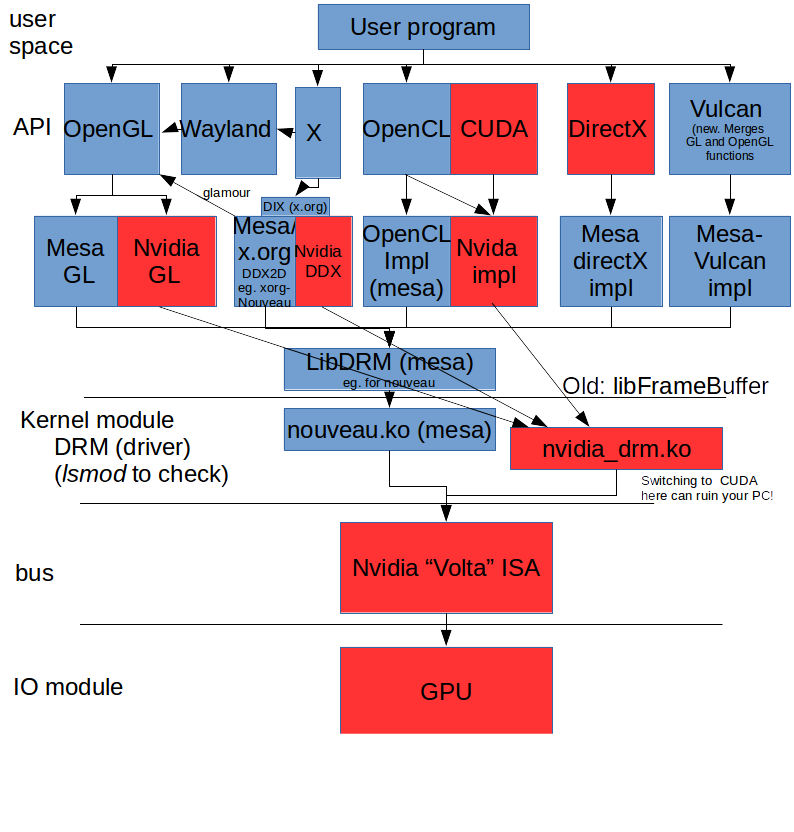
\includegraphics[width=7cm]{figs/graphicsStack.png}
\end{figure}

\section{Further reading}
\url{https://people.freedesktop.org/~marcheu/linuxgraphicsdrivers.pdf}

\url{https://blogs.igalia.com/itoral/2014/07/29/a-brief-introduction-to-the-linux-graphics-stack/}


\chapter{OpenGL (via SDL)}

OpenGL is the industry standard 3D graphics command language.  It provides an API containing commands which draw triangles and linesin 3D space, to render them under different lighting models, and to position the camera geometry around them.

In theory, the OpenGL API can be implemented in all kinds of ways, including fast graphics card hardware to take these commands and render them at blazing speed directly to a monitor. But also, for example, implementations might render drawings from the same commands onto bitmap images, vector graphics canvases, or even to robic spraycan or oil paintbrush manipulators.

Hence, to use the OpenGL requires an implementation library, such as Mesa, and usually a second library which links it to the screen or to a window in the operating system.   We will made use of the SDL (Simple Direct Layer) library as this link here.   SDL provides a graphics context which may be full-screen (eg for writing games) or windowed within the operating system.   


\subsection{SDL}

As modern systems operate from within a desktop window manager, which often gets implemented through OpenGL itself, some method is needed to prepare part of the screen and/or a window in the windowing system for the programmer's own OpenGL commands to run.  This is called a GL context.  It is provided by libraries such as SDL.   The programmer cannot give OpenGL commands directly because the window manager has already bagged the status of "master" of libDRM, and has instructed it not to take commands from anyone else.  SDL is given special permission by the window manager to pass its own commands (via the OpenGL implementations) to libDRM.  libDRM will then see that they coem from an allowed source and let them through to the kernel and GPU.

Simple DirectMedia Layer (SDL) is a cross-platform software development library designed to provide a hardware abstraction layer for computer multimedia hardware components including OpenGL graphics cards, and also keyboards and joysticks.  It is used in 3D games including 0AD, FreeCiv, Oolite, and in 2D games such as Secret Maryo Chnonicles and many others in Humble Bundles.  (Traditionally, a different link library, GLUT, was used. GLUT's programming model requires it to take full control of your program and communicate only through callbacks, while SDL keeps the user in control and assumes they will call its functions regularly. We consider the GLLUT model to be "rude" in takign over control, and this may conflict with other tools which also ask for control, such as ROS.  GLUT is considered old and dying.  Other altneratives include GLFW and pyglet for Python).

\lstinputlisting{snips/sdl_gl/sdlgl.cpp}
\lstinputlisting{snips/sdl_gl/CMakeLists.txt}

\subsection{GL/SDL Textures}

GL textures are simple bitmap images, ie. arrays of raw data in a specified format. (Such as 32bit RBGA color bytes).  SDL wraps these in a lihtweight struct which adds size and format infromation to the raw data. The raw data can still be accessed and passed to GL as an element in the struct (http://sdl.beuc.net/sdl.wiki/SDL_Surface):

\lstinputlisting{snips/sdl_image_texture/test.cpp}

\subsection{Video textures with CV/GL/SDL}

Suppose we are making a 3D video game set in a city and want to render a video of the Joker's threat to Gotham City on a giant screen on the side of a skyscraper.   Here we read frames usign OpenCV and push them into GL textures in real time.   This method is also useful fo AR if we want to just render a flat video image in GL -- it is done in exactly the saem way.  It is fast because the texture transfer is done via DMA on the GL command, so doesn't take up CPU time.

\lstinputlisting{snips/gl_video_texture.cpp}

\subsection{GL animation}

Once you have a context set up, you can apply any GL commands. The classic tutorial on pure GL programming is NeHe's website.  The classic reference is the OpenGL Red Book.

How OpenGL works intenrnall: graphics pipeline: https://fgiesen.wordpress.com/2011/07/01/a-trip-through-the-graphics-pipeline-2011-part-1/

\chapter{SDL 2D graphics and input}
eg for 2d platform games
we are using SDL1.2 (there is newer 2.0 now)

lazyfoo.net

Here is how to blit an image,

\lstinputlisting{/home/charles/Dropbox/linuxMultimedia/snips/sdlImageBlit/lesson01.cpp}

\section{Combining 2D and 3D graphics in SDL}
eg for Augmented Reality overlay!
blit + GL
done by blitting to texture ?

\chapter{Game Engines}
\section{2D}
pygame - built on SDL and OpenAL.  2D scene graph. Collision detection. Partial android version.

\section{3D}
Panda3D - unity-like - developed by Disney?
Blender game engine

\chapter{CAD}
FreeCAD
Blender

\section{Collada (dae) format}


\section{OpenSceneGraph (uses dae)}
B+trees (from GIS book?) - for collision detection

\section{ODE physics engine?}

\chapter{OpenCV}


\section{Reading and writing}

\lstinputlisting{snips/openCVcppCMake/videoWrite.cpp}
\lstinputlisting{snips/openCVcppCMake/CMakeLists.txt}

\section{Basic manipulations}


\chapter{Files and formats}

8 bit colouri = 256 color pallette. Usually with the palette defined in 24 bit in a header. (+ Old VGA has a fixed standard palette)
Standard 24 bit color = 1 byte for each of R,G,B. 32bit adds alpha byte too.  Nice to see and work with, human-readable in hex.

BGR (and ABRG) format for historical reasons. Used by GPU hardware, so libraries like CV follow it for speed.

Various color depths.

"convert" command - very versatile. eg. ps to png.


\section{Data formats}



\subsection{Bitmap (BMP)}

Windows standard. Header then raw RGB array data.

\begin{figure}
	\caption{}
	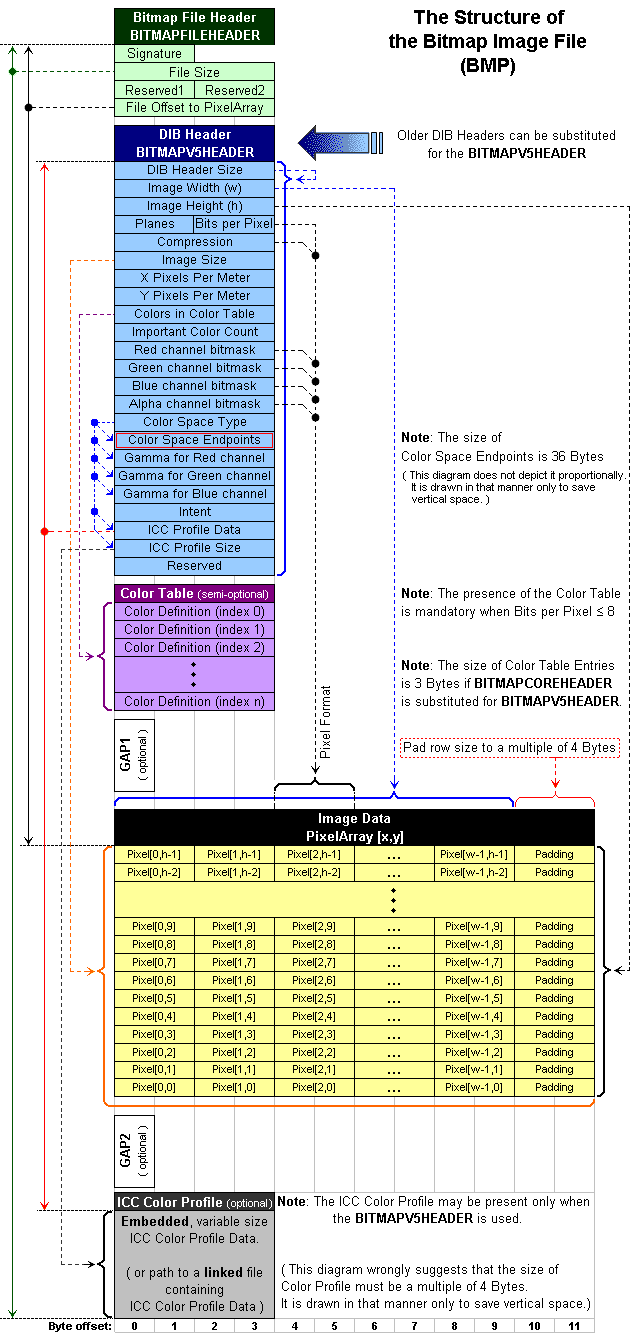
\includegraphics[width=7cm]{figs/BMPfileFormat}
\end{figure}



\section{ROS Image message}

header includes timestamps etc as well as img size and depth.


\section{Portable Network Graphics (PNG)}

compressed, like JPG. File made of chunks of labelled types.



\chapter{GPU OpenCL as graphics programming?}

\section{Architecture}

\section{Low level GPU ISA programming}

It is very rare to program GPUs directly in their own ISA.  Probably the only people who do this are staff at NVidia and staff and volunteers at Mesa who write the implementations for OpenGL and OpenCL etc.

NVidia's ISA is called PTX as is documented here,
http://www.nvidia.com/object/io_1195170102263.html

AMD's ISA is called R700 and is here,
ihttp://developer.amd.com/wordpress/media/2012/10/R700-Family_Instruction_Set_Architecture.pdf

An example program (for an R700 AMD card):

\begin{lstlisting}
00 ALU: ADDR(32) CNT(4) KCACHE0(CB0:0-15)   
0 x: MUL R0.x, KC0[0].x, KC0[1].x    
y: MUL R0.y, KC0[0].y, KC0[1].y
1 z: MUL R0.z, KC0[0].z, KC0[1].z
w: MUL R0.w, KC0[0].w, KC0[1].w
01 EXP_DONE: PIX0, R0
END_OF_PROGRAM
\end{lstlisting}

from:
https://stackoverflow.com/questions/27733704/how-is-webgl-or-cuda-code-actually-translated-into-gpu-instructions

to pass GPU binary via a CL function:
https://www.khronos.org/registry/OpenCL/sdk/1.0/docs/man/xhtml/clCreateProgramWithBinary.html


TODO how to call libDRM directly with the commands ?
\section{OpenCL setup}
We can choose the Mesa stack or a propriatory (eg. NVidia or Intel) stack, for the particular GPU type in our computer.

The Ubuntu nvidia stack can be installed via the Restricted repository, eg. nvidia-opencl-dev gets everything, and replaces the Mesa stack.  Then sudo apt install nvidia-cuda-toolkit to get CUDA and OpenCL APIs, cublas, cudnn, etc.

The mesa stack is harder ...  maybe easier in 16.04 ?
\begin{lstlisting}
/usr/lib/x86_64-linux-gnu/libOpenCL.so.1
\end{lstlisting}
ICD (Installable Client Driver) - Khronos tool to allow multiple implemenations of CL to coexist.
mesa-opencv-icd  apt package ?


\section{OpenCL programming}

Hello world in OpenCL:
\lstinputlisting{snips/cl/go.cpp}
\lstinputlisting{snips/cl/CMakeLists.txt}

(Cmake requres a manual link of libopencl.so.1 to libopencl.so before finding it).




\chapter{Applications}

GIMP
FreeCAD





\chapter{Vector graphics}

Vector graphics are 2D graphics which describe lines and shapes in terms of their points and connections in space rather than pixels. This means they can be rendered in different ways and scaled without pixellating.  There have been several formats and tools. The main standards today are pdf for text-heavy files, svg for graphic-heavy, and Cairo for creating these and others, including GUI renderings.

\section{Postscript vector graphics}

Postscript is an old but very alive vector graphics file format. Actually it is more than this: it is a fully fledged programming language.   Postscript files are human-readable programs which instruct a postscript device how to draw a vector image.  However full programming functionality such as for and while loops are not often used nowadays, and the postscipt "programs" encountered in the wild are usually just CAD-like lists of commands to move and draw with a virtual pen, like a 1908s LOGO turtle drawing.  It is common today to write programs in other languages (C, Python) which spit out postscript programs, rather that writing the programs by hand.

Example test.ps showing how to draw lines (open the file in a view such as GhostScript or send to a Postscript printer to view):
\lstinputlisting{snips/postscript/test.ps}

Encapuslated Postscript (eps) is a very minor extension to Postscript which adds a bounding box to the image; i.e. information about the size of the page or region in which it exists. This is commonly used to tell Latex how much space to leave around the egdes of figures. Simple tools convert ps to eps and back again.


\section{Portable Document Fomat (pdf)}

PDF is a newer vector graphics language based closely on postscript and eps.  It removes Postscipt's underused programming language facilities and keeps just the element descriptions, considering them to be static descriptions rather than programs.  (eg. a "line" is a description of the properties of a line entity rather than a command to "draw a line").  It adds the ability to wrap fonts inside the pdf file so they are guarenteed to be viewable with it - where postscript required the reader to have the right fonts on their computer.  PDF standard also defins a compression system which is often used to prevent human-reading and editing of the source as well as for actual compression.

\lstinputlisting{snips/pdfcut/pdfcut_cmd}


\section{SVG} format
PS and PDF have some ownshipship issues; SVG is a fully open standard for vector graphics files. Is is a flavour of XML and widely supported by web browsers:

\lstinputlisting{snips/postscript/test.svg}

\section{Cairo vector graphics API}

Cairo is an API for vector graphics drawing with many backends which can render these commands in many ways such as postscript and pdf files, SVG, on-screen GUIs, and OpenGL shapes.

Cairo's basic model includes:
Mask: defines a shape
Source: defines what's in the shape, e.g. a color, a bitmap, or a shading style.
Surface: the "canvas" being drawn on; this is implemented by the backends.

(This is a differnet model from those used by backends, however the backends do a lot of work to convert. eg. SVG uses a stylesheet model.  These models are important when we update drawings, e.g. in pure SVG we could wasily redraw all pictures on a website using red instead of green by changing the style. Using cairo, this change would be made at a higher level, in the drawing code, and the individual SVGs would not be able to inherit styles in that way any more. )

\lstinputlisting{snips/postscript/cairo/test1.cpp}

Cairo has many bindings including Python:

\lstinputlisting{snips/postscript/cairo/test1.py}

Cairo can also be used to draw in GUIs, as GTK provides a Cairo surrface type:

\lstinputlisting{snips/postscript/cairo-gtk/cairo-gtk.py}

\section{Fonts}

Fonts are special sets of vector graphics (for characters) which come wrapped with additional rules for how to display them together. (e.g. moving letters around to fit with one another, and responding to commands for resizing, italicizatio, kerning, etc.). In particular they are often displayed very small on pixel screen when reading text documents on screen, and come with special rules to display nicely at low resultions - such as use of grey pixels as hints to blend between black and white pixels - as well as printing nicely as pure black and white vectors.

Copy the .ttf file and paste it inside ~/.fonts folder, ie /home/username/.fonts folder. Create one if you dont already have one.

Now run

sudo fc-cache -fv


also Pango font rendering ?


\part{Audio}


\chapter{Audio hardware (sound cards)}

A sound card is really just a group of DAC (digital-anallog) converters, and indeed it is possible to make your own from any DAC such as found on Labjack, Software Defined Radios, or Arduino Duo. (Though not Arduino Uni, which fakes DAC using digital PWM).   Typically pro and consumer soundcards are optimised for certain features useful specifically for music production, including:
Low latency: a science lab DAC might not care about response time if it is just recording data; a musician cares a lot, especially if they are applying real-time processing to an instrument being played live, which needs to be just a few milliseconds latency.
Cost - for consumer cards. Limit number of channels eg. to stereo in an out; whil science lab recorders may have hundreds or thousands of channels.
Quality - optimise for audio signals which run in audible frequency ranges (48kHz recording is the pro standard; representing Nyquist rate for human perception of half of this, 24kHz) and have known (eg. 24 bit is the pro standard) bit-depth perceptual detetions.

Sound card hardware typically consists of a ring-buffer for each channel, and DAC hardware which reads or writes to/from it. A ring buffer maintains a pointer to the next location to write, and wraps the storage around the ring so it doens't run out of storage. The buffer size provides a tradeoff between latency and dropouts. Small buffer means low latency but risks dropouts.  We can also choose the bit depth of the audio.

Sound cards, like graphics cards, connect to the computers system bus. They are less bandwidth hungry than video so are usually found on a bus hanging off of Southbridge, such as PCI for internal cards, or USB or Firewire for external cards.  PCI and Firewire are true busses (eg. Firewire devices can be daisy chained as they all see the full content of the bus) while USB is not a bus put a point-to-point connection.

Sound card hardware APIs vary by manufacturer, and like GPUs their details may be propriatory and known only to the driver writers inside the company, who then make a software API available. As with GPUs the hardware API are then reverse engineered by open source driver writers.  They typically (?) consist, like GPUs, of device-specfic commands sent as data writes and reads (i.e. commands which initiate data transfers to/from main memory and/or CPU?).

(In theory: APIs could include GPU texture style DMA transfers with main memory, I'm not sure if anyone needs or does this though? Might that be interesting?  Are there speeds to be gained by reading direct to CPU rather than memory first? Is this already done?)

\chapter{Audio software stack}

\begin{figure}
  \centering
  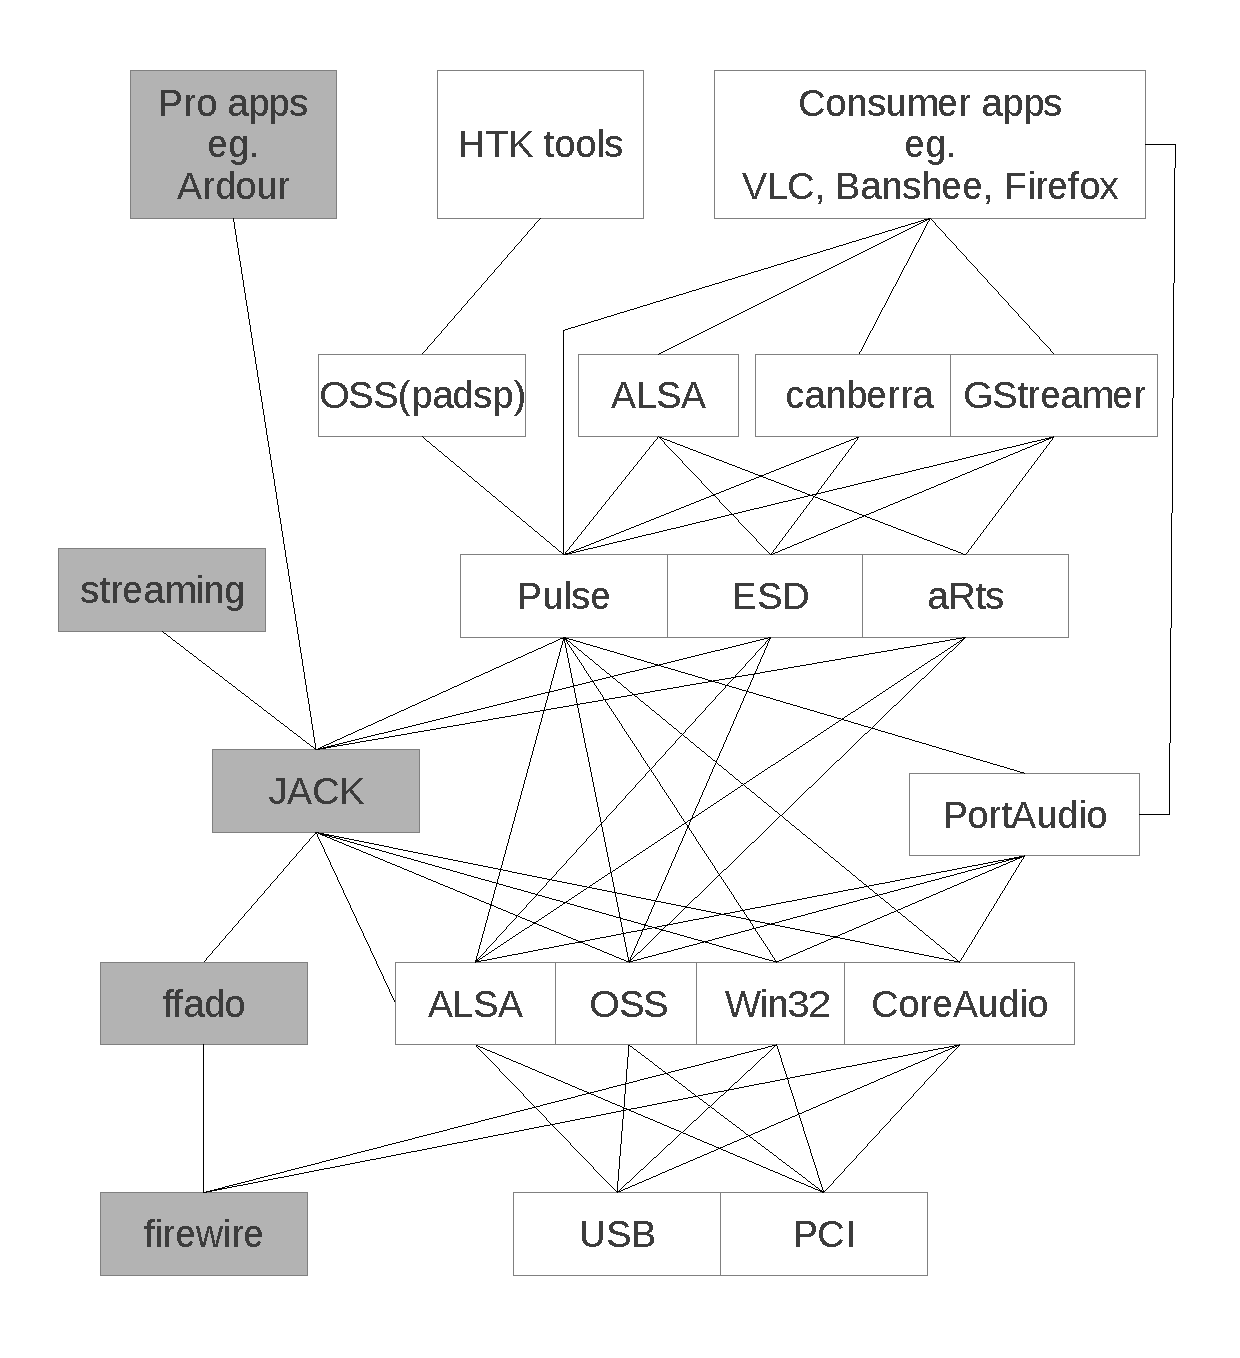
\includegraphics[width=\columnwidth]{figs/linuxaudiosystem-studio.pdf}
  \caption{Audio system for recording.}
  \label{fig:audio-rec}
\end{figure}

Fig. \ref{fig:audio-rec} outlines the current Linux audio system and highlights the parts used in our stack.  The Linux audio architecture has grown quite complex in recent years, with multiple ways of doing things competing and improving.

Historically, the OSS API and implementation was developed for Linux in the early 1990s, focused initially on the Creative SoundBlaster cards then extending to other PCI and USB devices.  It was a locking system which allowed only one program at a time to access the sound card, and lacked support for modern features such as surround sound. It allowed low level access to the card, for example by $\tt cat audio.wav > /dev/dsp0$.  

The ALSA API and implementation was designed as a modern replacement for OSS, and is used on most current distributions to control PCI and USB soundcards.  It does not handle Firewire cards. It is also a locking system.

PortAudio is an API with multiple backend implementations that abstract both OSS and ALSA, as well as sound systems of non-free platforms such as Win32 sound and Mac CoreAudio, created to allow portable audio programs to be written.  

Several software mixer APIs and implementations were then built to resolve the locking problem for consumer desktop applications, including PulseAudio, ESD and aRts.  Like graphical window managers which enable applications to share the screen, these allow multiple applications to request audio channels at the same time, and handle mixing them together to send to a single physical audio device.  Some of these mixers grew to take advantage of hardware mixing provided by some sound cards, and to provide features such as network streaming.  They provided their own APIs as well as emulation layers for older (or mixer-agnostic) OSS and ALSA applications.  (To complicate matters further, recent versions of OSS4 and ALSA have now begun to provide their own software mixers, as well as emulation layers for each other.)  Many current Linux distributions including Ubuntu 11.10 deploy PulseAudio running on ALSA, then also include an ALSA emulation layer on top of Pulse to allow multiple ALSA and Pulse applications to run together through the Pulse mixer.  Common media libraries such as GStreamer (which powers consumer applications such as VLC, Skype and Flash) and libcanberra (the GNOME desktop sound system) have been developed closely with PulseAudio, increasing its popularity.  For writing a new desktop applicaiton with audio, we probably want to use the ALSA API, and link it to the ALSA emulation layer on Pulse.  (Or if we are sure that we want to take ove the whole sound system, for example writing a pro audio application, then the same ALSA API can be linked directly to the low-level ALSA library itself without pulse.)

The JACK system is an alternative software mixer designed for pro-audio, multi-process work which relies on very low latencies and minimal drop-outs, such as Digital Audio Workstation applications.  Like the other soft mixers, JACK runs on many lower level platforms -- usually ALSA on modern Linux machines.  The bulk of pro-audio applications such as Ardour, zynAddSubFx and qSynth run on JACK.  JACK also provides network streaming, and emulations/interfaces for other audio APIs including ALSA, OSS and PulseAudio.  (Pulse-on-JACK is useful when using pro and consumer applications at the same time, such as when watching a YouTube tutorial about how to use a pro application.  This re-configuration happens automatically when JACK is launched on a modern Pulse machine such as Ubuntu 11.10.)  JACK applications have standard input and output channels which can be patched together to form complex musical symthesis and processing chains. (Such as, using an audio drum output signal as a side-chain to control a Eric Prydz-style compressor.)

LADSPA is a weaker API which also enables plugins to be chained, similarly to VST plugins on Windows/Cubase, and which includes APIs for graphical interfaces with control dials and for more easily saving their state as part of a DAW setup.

FFADO is a driver for pro Firewire devices, and includes JACK and other interfaces as well as its own interface and command-line tools for basic recording and playback.  (Until recent USB3, Firewire was the "pro" choice; USB3 has now caught up and should be the new pro standard.)


\chapter{ALSA}

ALSA is a single-process API.  Its main implemention is a low-level one which takes full control of the soundcard, and which is used, for example, by higher level mixer applications.  The API is however also re-implemented at an even higher-level, where mixers emulate multiple ALSA soundcards and make them avaiable to applications.  They then do the mixing and send the result out to the original low level ALSA.  Thus learnign ALSA is useful for programming at both the audio system and the audio application level;

See ALSA tutorials:
http://users.suse.com/~mana/alsa090_howto.html

\section{input}


\section{output}


\chapter{Spatial audio: OpenAL}

\chapter{JACK}

\section{setup}
\url{http://jackaudio.org/faq/linux_rt_config.html}

\begin{lstlisting}
    jackd -d alsa - r48000 -p128 -n2  -P hw:1,0 -C hw:1,1    #works for mic in socket1 of MAUDIO, and for MAUDIIO playboack (not for mic in s2?)

	jackd -dalsa -dhw:0 -r48000 -p128 -n2  #INTERNAL soundcard (not -p64 kills ard3)
	
	killall -9 jackd

qjackctl: (not needed if use JACK cmd above)
	interface (default) (greyed out)
	in dev: hw:1,1
	out dev: hw:1,0	
	chs 2 in 2 out
	128 frames.
\end{lstlisting}

\section{JACK tools}
NB we need to record form the nonstandard hw1,1 , not the default hw1,0:

\begin{lstlisting}
 /usr/bin/jackd -P65 -u -dalsa -r48000 -p128 -n2 -Xseq -D -Chw:1,1 -Phw:1,0 -i2 -o2    #works (and in qjackctl)

killall -9 jackd			#to kill
ecasound -f:16,2,48000 -i jack,system -o rec.wav  			 #record -- not working** (16bit,2ch,48kHz)
ecasound -i output.wav -o jack,system 					 #playback

meterbridge 1   #to open a test app - use qjackctl to connect
\end{lstlisting}

\section{Configuring JACK for pro audio}

For example: Our DAW was a relatively low-power Intel E8400 (Wolfdale) duo-core, 3GHz, 4Gb Ubuntu Studio 11.10-64-bit machine.   Ubuntu studio was installed directly from CD -- not added as packages to an existing Ubuntu installation -- this gives a more minimalist installation than the latter approach.  In particular the window manager defaults to the low-power XFCE, and CPU-hogging programs such as Gnome-Network-Monitor (which periodically searches for new wifi networks in the background) are not installed.

The standard ALSA and OSS provide interfaces to USB and PCI devices below, and to JACK above.  However for firewire devices such as our Pre8, the {\tt ffado} driver  provides a {\em direct} interface to JACK from the hardware, bypassing ALSA or OSS.  (Though the latest/development version provides an ALSA output layer as well.)   Our DAW uses {\tt ffado} with JACK2 (Ubuntu packages: {\tt jack2d, jack2d-firewire, libffado, jackd, laditools}.  JACK1 is the older but perhaps more stable single-processor implementation of the JACK API) and fig. \ref{fig:jack-settings} shows our JACK settings, in the {\tt qjackctl} tool.  Note that the firewire backend driver (ie. {\tt ffado}) is selected rather than ALSA.

It is important to unlock memory for good JACK performance.  As well as ticking the unlock memory option, the user must also be allowed to use it, eg. {\tt adduser charles audio}.  Also the file {\tt /etc/security/limits.d/audio.conf} was edited (followed by a reboot) to include

{\tt @audio - rtprio 95 }

{\tt @audio - memlock unlimited }

These settings can be checked by

{\tt ulimit -r -l}.

The JACK sample rate was set to 48kHz, matching the Pre8s.  (This is a good sample rate for speech research work as it is similar to CD quality but allows simple sub-sampling to power-of-two frequencies used in analysis.)

Fig. \ref{fig:jack-connect} shows the JACK connections (again in {\tt qjackctl}) for our meeting room studio setup.  The eight channels from the converter-mode Pre8 appear as ADAT optical inputs, and the eight channels from the interface-mode Pre8 appear as `Analog' inputs, all within the firewire device.  Ardour was used with two tracks of eight channel audio to record as shown in fig. \ref{fig:ardour}.



\begin{figure}
  \centering
  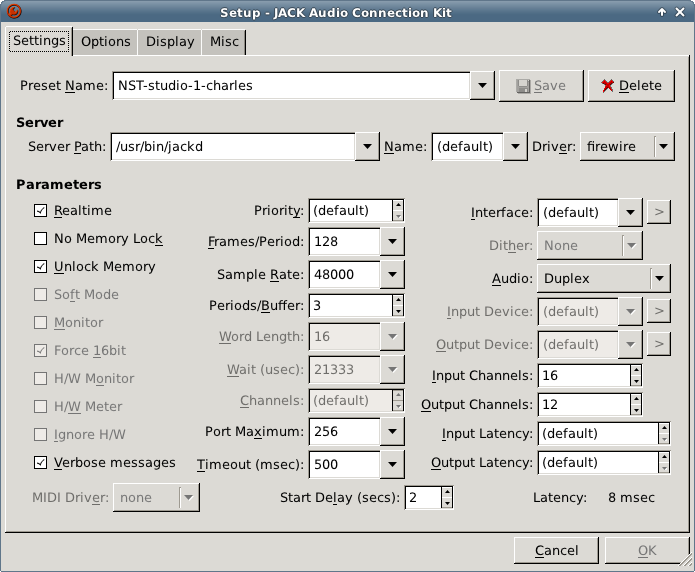
\includegraphics[width=\columnwidth]{figs/jack-settings.png}
  \caption{16 channel recording JACK settings.}
  \label{fig:jack-settings}
\end{figure}

\begin{figure}
  \centering
  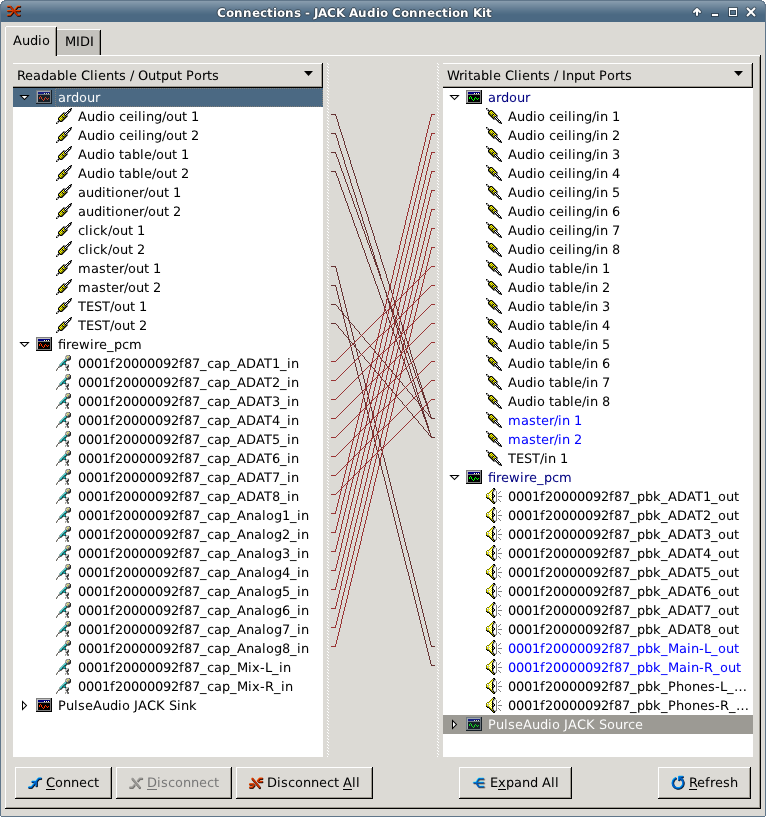
\includegraphics[width=\columnwidth]{figs/jack-connect.png}
  \caption{16 channel recording JACK connections.}
  \label{fig:jack-connect}
\end{figure}

\begin{figure}
  \centering
  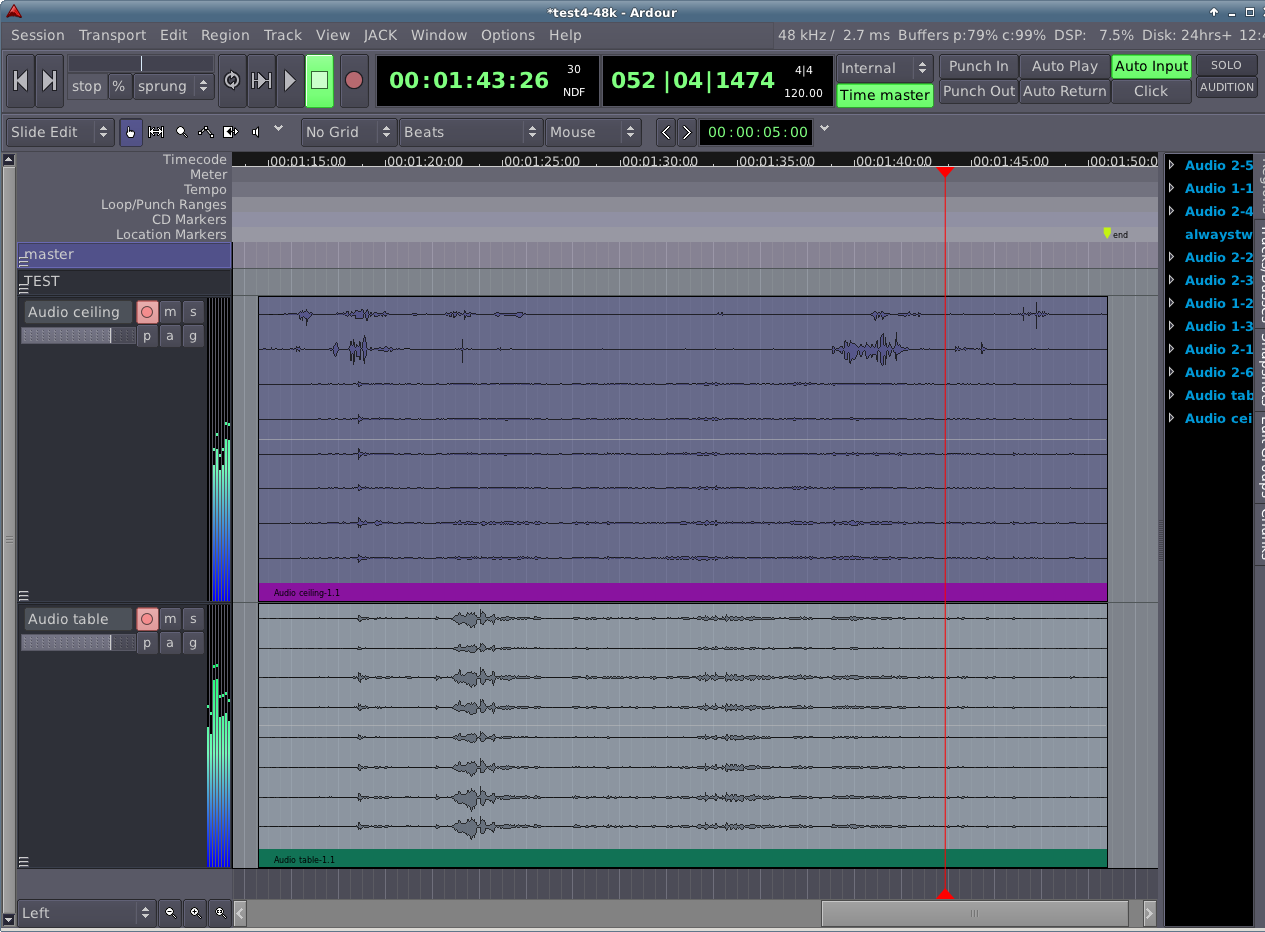
\includegraphics[width=\columnwidth]{figs/ardour.png}
  \caption{16 channel meeting room recording in Ardour, using two 8-channel tracks.}
  \label{fig:ardour}
\end{figure}


\subsection{Example: MAUDIO USB card}
    inputs:
	signal dials: -40db control.   Pad: extra -20db.
    flow model:
	all inputs have direct JACK outputs
		the box also has a line out and a phones out
	A/B button-out :patches line out to phones when OUT(A);  
		(spdif to phones when button-in, B)
		so ALWAYS button-OUT if not using any SPDIFs
	Mix: Left: live inputs to phone.  Right: PC to phones
		should be all-right
	Output: volume of line out
	Level: volume of phones
	gtr: inst, vol at 45deg north east

	#NB sampled audio goes out of the MAUDIO through  hw:1,1.  That's nonstanard, defaults are usually hw1,0.  So need to set to listen to hw:1,1.

	#2015: on XPS machine -- need hw2,0 OUTPUT and hw2,1 INPUT (different!)  mich ch 1



\chapter{LADSPA}


\section{MIDI}

live

files



\chapter{Music notation}

\section{MusicML}
Is a (not very) human read-writable XML standard backed by many large companies and projects, including beign the standard for music notation on Wikipedia.

(Unliek Lilypond) it would not be nice to write by hand. It is better to use a graphic free editor such as MuseScore.

Can be converted to lilypond for engraving with musicxml2ly tool (ships with Lilypond). It is not usually possible to go the other way. Hence editing should be done in MusicXML and only exported one-way to Lilypond for engraving.  Don't write in Lilypond as its not transferrable out. (until someone writes a converter).

Due to its horrific XML verbosity (several lines of text to describe each note) there is a zipped version included in the specification. As with other XMLs, the philosophy is to be human readable but verbose then worry about compression separately.


Ontology of MusicXML: harmony changes and section names are discrete events put into measures at points.  Lyrical sylablus are tagged to individual notes. (which make it hard to write lyrics separetly from the music; but forces the music to have the correct maps to the notes.  As usual, MusicXML is not for composing in, it's a low-level description of the notes. Might want to use some other ABC like notation for lyrics and compile to here?)

\section{MuseScore}
Is standard opensource graphical MusicXML editor. Has its own format too.   

Has semantic guitar chords (appear as 'harmony' objects in XML). Transposable (Notes->Transpose). Can play back as MIDI. To split music into sections eg. verse, chorus, use a 'section break', show by 'new system' flag in the XML, plus add>text>rehearsal mark. (The mark names a point not a segment; but we can interpret as namign the segment up to the next mark or end.)

To enter: press N for note entry mode. Press number 1-8 for duration. Type note letter name C,D,E etc or 0 for rest. They assume the current octave.  Cursor keys to move back and forward in time, and to move notes up and down. Also mouse entry.

MuseScore.com has a large library of standard music to download, eg. Beatles, Mozart, in own and MusicXML formats.

\section{ABC notation}

A common standard for folk music especially.   Words are paired with {\em lines} of music, usign hyphens and ties to link them to the notes.

Can be converted to (and partially from?) MusicXML.

Lilypond format is based on it but extends it a lot.

Maybe a nice format for MusicHastie-like systems to all standardize upon.


\section{Lilypond engraving}
Lilypond is like Latex for music scores.  It names both a file format and a program.  It creates extremely high-end, professional "engravings" of scores, including fine details equivilent to Latex's kerning and ligatures. Such as tweaking the exact size of note heads and stems, setting stem directions, and hundreds of other small rules passed down from centuries of beautiful score engraving tradition.   The Lilyond program is not an editor and works from a latex-like source file specifying the musical, but not graphical, objects, such as bars, notes, and time signatures. These files can be written by hand or by an editor program such as Denemo (see below). These files do not contain any high level semantic information and they do not show relationships between simultenoys staves (e.g. that a note in one staff is occuring at the saem time as in another) or enable transpoition -- they only represent the low-level musical note content needed for engraving. So you probably don't want to cide directly in LilyPond files. You want to code in some higher level representation then use another program to export it to Lilypond format. 

LilyPond can however do basic transposition from within its code -- usign a transpose command and environment. This is sufficient for quick conversions eg. for Bb jazz isntruments. But not going to be able to do hierarachical stuff.

eg. to write a Schenkerian composition program: use its won format and notation at high level; export to MusicXML; convert to LilyPond; engrave.

Sample Liypond source:
\lstinputlisting{snips/lilypond/test.ly}

To isntall and compile to pdf:

\begin{lstlisting}
sudo apt-get install lilypond
lilypond test.ly
\end{lstlisting}

Notations:
\begin{lstlisting}
c4 d4 e4 f4  : crochets. 4 means quarter note.
r1 r2 r4 r8  : rests
a4. dotted quarter-note
ds4 : d sharp
a,4 a'4 : octave registers CHANGES. assumes all followign notes in same register.
<c4 e4> : notes together
(c4 e4) : slur notes
\repeat volta 2 { c1 | e1}  : repeat section
c4^"super" e4_"sub" : text above and below note 
\end{lstlisting}

Dynamics are considers as additional over staves.  (LilyPond's name is a pun on an old MIDI editor, RoseGarden).

\subsection{Denemo score editor GUI}
Is designed specifically as a front end to LilyPond, and is to LilyPond as LyX is to Latex.  A what you see if what you mean GUI with its own quick, cheap and chearful interactive graphical screen display, which gets swapped for the advanced engraver when we are done.

Includes human input + assign rhythms to the hummed pitches.

Curosr updown pitch, or type letter name (register nearest to cursor pitch).  Int number keys (use keypad) for durations.

Generally we don't want to compose or edit in Denemo because then we are stuck in Lilypond world and can't get back to MusicXML.  We might thus use Denemo to add really fine grained engraving detail to a score done in MuseScore, just for priting..

(Does not yet export MusicXML but may do soon? CHECK?)

\sdubsection{Frescobaldi}
FrescoBaldi - a Lilypond editor which does have MusicXML output? Tis one is not pointy clicky like LyX, is like TexPad, editing the raw lilypond code but with tools to autocompile and display etc.


\chapter{Audio file formats}

\section{wav}

header + raw bytes. (raw = Pulse Code Modulation) eg. 32 bit audio = 4 bytes per sample, from linearly spaced possible values. (32 bit here is the 'bit depth').
NB 4Gb limit? still dont know how to fix this/ repair from header.

Since recently - wav also supports floating point representations (which avoid clipping but require more computation).

\section{vorbis}
used in ogg containers.

TODO how to edit meta-data artist, year etc.

\section{AAC}
Audio format often used in mp4 containers along with videos.

\sectin{FLAC}
Lossles.

\chapter{Tools}
\section{Sox and soxi}
Sox is the swiss army knife of the audio command line. Its friend soxi gives information about audio files.
\begin{lstlisting}

	sox k.wav -n stat   #see length(seconds)
	sox in.wav out.wav trim start_time dur			
	sox in.wav out.wav pad start_pad_sec end_pad_sec

	sox ts.wav -b 16 output.wav rate -s -a 48000 dither -s    #upsample
	sox mono.wav -c 2 stereo.wav                              #make stereo fm mono (JACK cares a lot about right types here)

	#delay and weighed mix.  -p is used in place of output fn, to pipe out.
	sox -m -v 0.9 a.wav   -v 0.5 '|sox a.wav -p pad 1' out.wav    #in seconds
	sox -m -v 0.9 a.wav   -v 0.5 '|sox a.wav -p pad 1s' out.wav   #in samples

	#lima
	sox -D -m -v 1 -t sox "|sox a.wav -p pad 0s trim 0 5s"      -v 0.5 -t sox "|sox a.wav -p pad 1s trim 0 5s"  out.wav
 
	#equiv to (as "-p" subs to "-t sox -" and "-" is the pipe out)
	sox  -m -v 1 -t sox "|sox a.wav -t sox - pad 0s trim 0 5s"      -v 0.5 -t sox "|sox a.wav -t sox - pad 1s trim 0 5s"   out.wav
	
	#piping out of sox
	sox -m -v 0.9 a.wav   -v 0.5 '|sox a.wav -p pad 1s' -t wav - | less    #WARNING about wav header though

	#pad and trim
	sox Array1-01.wav -p pad 0s trim 13437440s 104800s  o2.wav

 soxi  /share/spandh.ami1/asr/dev/mtg/ac/exp.mdm/exp/lima/pylima/out/testRun/AMI-S1000B_m4016_083984_084639/iter1/mix.wav

Input File     : '/share/spandh.ami1/asr/dev/mtg/ac/exp.mdm/exp/lima/pylima/out/testRun/AMI-S1000B_m4016_083984_084639/iter1/mix.wav'
Channels       : 1
Sample Rate    : 16000
Precision      : 32-bit
Duration       : 00:00:06.55 = 104800 samples ~ 491.25 CDDA sectors
File Size      : 419k
Bit Rate       : 512k
Sample Encoding: 32-bit Signed Integer PCM

\end{lstlisting}

\section{ALSA command line tools}
\begin{lstlisting}

aplay -D hw:0,0 stereo.wav   #PC
aplay -D hw:0 stereo.wav     #PC
aplay -D hw:1,0 stereo.wav     #USB
aplay -D hw:1,1 stereo.wav     #silent (spdif?)

arecord -f cd -D hw:1,1 g.wav           #works**

\end{lstlisting}

\section{Musical descriptor features}
Queen Mary tools?


\chapter{Music synthesis}


\section{Musical descriptor features}
Queen Mary tools?
\chapter{Speech synthesis}

festival


\chapter{Speech recognitions}

kaldi?


\chapter{Applications}

list best LADSPA plugins?

LMMS

\section{Ardour 3}

just create new audio track, should be already to record. 
	(right click in track space, add track)
	(dont need to add audio bus patch) 
	for second and more tracks:
		might need to set to hardware in 1 vs 2
			use icons in top right under "Audio2"

flow model:
	jack,system is conencted auto to the Ardour Master
	the master is connected to any track with record enabled.

region = one segment of wav or midi

SPACE: 		play/stop
SHIFT-SPACE:  	play and record  
SHIFT-R:  	en/diable record (while playing)
(CTL-SPACE: 	stop and forget record)

PUNCH markers are set by ctrl-drag in marker field. 
	Enable puch IN OUT at top right of screen. (under DSP) 
	Press [ to set markers + drag them
	Start record (not just play)
	NB this records NEW WAV FILE doesn't destory old one
 
L: 	en/disable loop play
	works similar to punch, using ] instead of [
	each version is separate WAV, keep old ones	

cursors: 	move to start/end of regions
shift-cursors: 	cue (use spa  ce to stop)
ctl-cursor 	move to marks (CF set, was keypad)

HOME/END goto start/end

6: Auto-Return enable: back to play start location (after play or rec)
7: clicks

to0 SPLIT: select region, position playhead, press S


ARDOUR editing
	S split region at edit pount
	use trim bar (region name area) to crop left and right ends

ARDOUR CONFIGS:
	preferences - default dir

\section{ZynAddSubFX}

musichastie?


\part{Video}


\chapter{Video architecture}

Multimedia comes in various kinds of streams. Streams may contain
video or audio or other things. These may be compressed with codecs,
eg h264,theora. Combining streams eg audio+video is multiplexing.
Demupliplexing is seprate from decoding. Streams can be passed over
realtime protocols such as RTP or stored in container files such as
mp4,ogg. problem with compressing video is that it introduces lateny,
some compressions require knowledge of future frames, eg MP4. Others
are designed for live use eg H264. 

Rough rule for video CPU usage: on a 2017 laptop, coding or decoding one video does not start the CPU fan; doing two or more does. (Possibly they are designed to this, as watchign a single video as a consumer is much more common that doing anything fancier.)  Consequences: if we want to run two programs than run on the same video stream, the fan is needed. They must either share an encoded stream and each run decoders, so we have two decode processes; or decode one but then stream high-bandwidth raw images around, which also starts the fan! Having the fan on for long periods has previously melted by CPU glue and required sending my laptop to Germany to have it replaced so is not recommended.

eg. playing 2 hi-res youtubes in cinema mode at once takes about 200\% CPU and starts the fan. (NB youtube does many clever things such as ceasing to download video when the window is not visible; need to open the windows for a full test.)

IP cameras - streaming.  vs. save to container files.

\chapter{Video4Linux (V4L)}

is a standard API for video devices such as webcams, plus some drivers
implementing it.

API devices appear as files at ls /sys/class/video4linux/ which can
be accessed eg. via pythonCV: cv2.videoCapture(3) 

v4l2-ctl: gives low level info and setting for USB camera hardware
typically GUI tools are calling into it to change camera settings

has many useful help options, see --help 

get current settings: v4l2-ctl --device=/dev/video0 --get-fmt-video

eg to set image size and codec: v4l2-ctl --device=/dev/video0 --set-fmt-video=width=800,height=600,pixelformat=1

logitech C920 has onboard codecs: YUYV -- splits up luma (Y) and croma
(Cr and Cb red and blue diffs) and downsamples chroma a bit (YUV 4:4:2)
MPEG H264

ask for available frame rates: v4l2-ctl --device=/dev/video0 --list-frameintervals=width=640,height=480,pixelformat=YUYV


\section{Loopback}
\label{loopback}

Loopback is a system which allows you to create virtual video devices
in V4L, so that other applications may access them just as if they
were real devices. Like real devices they appears in /dev/videoX.

Loopback module must be installed then enabled with:

\begin{lstlisting}
sudo apt-get install v4l2loopback-dkms 
sudo modprobe v4l2loopback
\end{lstlisting}
This creates virtual devices /sys/class/video4linux/video1 and /dev/video1 which behave like local webcams. For example they can be opened in OpenCV:


\chapter{Video formats (codecs)}

\section{raw images}
Individual frames may be stored or transported, either as uncompressed images themselves (bmp) or as compressed images (png/jpeg). However much better compression comes form considered the frames in sequence and compressing accordingly. eg. often the camera does not move and large areas of background do not change over time.

Images have pixel formats. Traditionally, still images are stored in RGB (or similar, BGR, or RGBA) as three (or four) bytes per color channel.  However it is more common for video images to use different pixel formats.  This could be HSV (hue saturation value) or more commonly, YUV format, which is a similar idea to HSV.  Like RGB, which can be various bit-depths (eg. 24bit, 8bit), YUV also comes in different depths and flavours. YUV also has nice compression properties which make it popular now.  Y=luma (overall brightness); U and V are 2D chromas. (Historically: its was nice for sharing streams for black-and-white and color TVs, such as in USA PAL analog broadcasts, because the luma channel looks good by itself in B+W.)

\section{theora}
Open format video codec used in ogg containers.

\section{h264 (aka. MPEG4-part 10; MPEG4-AVC}
Used in Freeview and Freesat Digital TV; Skype, Bluray, Youtube, inside mp4 containers, CCTV cams.
heavily patenteted but allowed for gratis use in some cases.
Uses image subblocks;  motion prediction
http://iphome.hhi.de/wiegand/assets/pdfs/h264-AVC-Standard.pdf

\section{MPEG2 video (MPEG2-Part2; h.262)}
used in most DVDs.    (don't confuse with MPEG2 container which also has various audio formats (MPEG2-Part3) and system control protocol MPEG2-Part1/h.222).

\section{MTS}
MTS is a video codec found on portable digital cameras and phones.
Here is a conversion method using mencoder:

\begin{lstlisting}
sudo apt-get install build-essential subversion zlib1g-dev
	svn checkout svn://svn.mplayerhq.hu/mplayer/trunk mplayer
	cd mplayer
	./configure
	make
	sudo make install
	mencoder 00001.MTS -o 1.avi -oac copy -ovc lavc -lavcopts vcodec=mpeg4:vbitrate=10000 -fps 50 -vf scale=1920:1080
\end{lstlisting}

\section{AV1}
AV1 is a 2018 video codec designed fully open source and patent free to improve and replace h264 (MP4part10).

\chapter{ffmpeg}

ffmeg is a simple command line tool for performing quick, small operations on media files.

transcode to open source everything (ogg+vorbis+theora; very slow):
\begin{lstlisting}
ffmpeg -i in.mp4 -acodec libvorbis out.ogg
\end{lstlisting}

extract section: 
\begin{lstlisting}
ffmpeg -ss 00:00:05.123 -i in.mp4 -t 00:01:00.00 -c copy out.mp4 
\end{lstlisting}

extract frame as image,
\begin{lstlisting}
ffmpeg -ss 00:12:58 -i in.mp4  -vframes 1 -q:v 2 out.jpg
\end{lstlisting}

Get video file info,
\begin{lstlisting}
ffprobe -show\_streams -i \textasciitilde{}/data/qb/NorwichLeeds1280.mp4
\end{lstlisting}

Speedup playback of video 
\begin{lstlisting}
ffmpeg -r:v \textquotedbl{}480/1\textquotedbl{}
-i in.mp4 -an -r:v \textquotedbl{}12/1\textquotedbl{} out.mp4
\begin{lstlisting}

Split video into image frame files: 
\begin{lstlisting}
ffmpeg -i corinthian\_raw\_images.avi -f image2 frames/frame-\%3d.png 
\end{lstlisting}
(start time and duration args; can be 00:00:00.000 format, or seconds as 00.000. NB only splits to nearest keyframes, unless omit copy to transcode)

downsample,
\begin{lstlisting}
ffmpeg -i in.mts -r 30 -s 960x540 out.mp4
\end{lstlisting}

downsample resolution: 
\begin{lstlisting}
ffmpeg -i in.avi -c:a copy -c:v libx264 -crf 23 -s:v 640x360 output.mp4
\end{lstlisting}

trim:
\begin{lstlisting}
ffmpeg -i in.avi -vcodec copy -acodec copy -ss 00:00:00 -t 00:00:04 out.avi
\end{lstlisting}



\chapter{GStreamer}

GStreamer a Linux system for media streaming, within and between computers. It is based on small modules (processes) which are 'piped' together similarly to UNIX pipes.  Like ROS this allows everything to run as separate processes. Unlike ROS, GStreamer is targetted at efficiency which includes use of containers and codecs for everything. In ROS we pass messages of raw image data in video. In GStreamer we can stream coded compressed video for speed and efficiency.  This means we need to consider container and codec modules in the pipelines.

\section{as command line tool}

GStreamer is sometimes used as a competitor to ffmpeg to perform small command line media editing tasks such as cutting and splicing video and audio streams. It is more powerful and harder to use than ffmpeg because of its pipeline abilities.  It would be a good habit to get used to using GStreamer instead of ffmpeg even for small tasks, so that it becomes regular and easy to use for large ones.

GStreamer requires modules (plugins) to go in the pipelines. The main ones are distributed in packages:
 Base: solid stable simple ones used by many other tools;
 Good: solid stable more specific ones, eg. theora codecs.
 Ugly: solid stable but with patent issues, eg. reverse engineering of propriatory codecs.
 Bad: In-development, unstable, bleeding-edge, for use at own risk.

We are using version 1.0 for everything (0.10 also exists) Modules
are binary (Cpp) executables, implementing standard API. (Like LADSPA
- but not as real time? eg including buffering).

There are modules for reading and writing to/from v4l devices. eg. stream things
into new virtual v4l devices for others to read. also UDP data stream
sources and sinks. v4l is a minority sport though as gstreamer has
its own internal appsrc and appsinks.

We can give transport control commands to jump to points in streams using an additional interface.

\subsection{Examples - local streams}

(\textquotedbl{}!\textquotedbl{} makes the pipe, like unix \textquotedbl{}|\textquotedbl{}
but called a \textquotedbl{}pad\textquotedbl{} rather than \textquotedbl{}pipe\textquotedbl{})

Basic copy a source file to a sink file: 

\begin{lstlisting}
gst-launch-1.0 filesrc location=in.mp4 ! filesink location=out.mp4
\end{lstlisting}

Play an mp3:

\begin{lstlisting}
gst-launch-1.0 filesrc location=in.mp3 ! decodebin ! autoaudiosink
\end{lstlisting}

Play mp4 video 
\begin{lstlisting}
gst-launch-1.0 filesrc location=in.mp4 ! decodebin ! autovideosink
\end{lstlisting}
(decodebin is a complex plugin which detects the video filetype and automatically constructs a whole series of modules specific to its type to decode it.)

Show TV test card source,
\begin{lstlisting}
gst-launch-1.0 videotestsrc ! autovideosink
\end{lstlisting}

Extract a segment of a file, recode, and send to another file (not
working) 

\begin{lstlisting}
gst-launch-0.10 gnlfilesource location=in.mp3 start=0
duration=5000000000 media-start=10000000000 media-duration=5000000000
! audioconvert ! vorbisenc ! oggmux ! filesink location=out.ogg
\end{lstlisting}

Decode a file and stream raw video to a file, 
\begin{lstlisting}
gst-launch-1.0 filesrc location=in.mp4 ! decodebin ! filesink location=out.mp4
\end{lstlisting}

Read from webcam, downsample, and view:
\begin{lstlisting}
gst-launch-1.0 v4l2src device="/dev/video0" ! video/x-raw,width=640,height=480 ! autovideosink
\end{lstlisting}

Split a source into multiple sinks using "tee" (like in Unix "Tee"; named after the shape of the letter "T" where a signal from below splits into left and right copies.),

\begin{lstlisting}
gst-launch filesrc location=test.mp4 ! tee name=tp tp. ! queue ! filesink location=out2 tp. ! queue ! filesink location=out2
\end{lstlisting}

\subsection{Examples - network streams}

Stream to RTP over UDP port (e.g. to broadcast a live video stream on the net):
\begin{lstlisting}
gst-launch-1.0 filesrc location=in.mp4 ! decodebin ! x264enc ! rtph264pay ! udpsink host=127.0.0.1 port=9001
\end{lstlisting}
This works by decoding the local file, encoding it in the desired codec, then containerising (payloading) it as RTP, then sending over a lower-level UDP link.

Version to lowwer quality and reduce latency (?):
\begin{lstlisting}
gst-launch-1.0 filesrc location=in.mp4 ! decodebin ! x264enc pass=qual quantizer=20 tune=zerolatency ! rtph264pay ! udpsink host=127.0.0.1 port=9001
\end{lstlisting}

To read the stream into GStreamer,
\begin{lstlisting}
gst-launch-1.0 udpsrc port=9001 ! "application/x-rtp, payload=127" ! rtph264depay ! avdec\_h264 ! videoconvert ! xvimagesink
\end{lstlisting}

From a remote RTP stream (e.g. an IP camera),
\begin{lstlisting}
gst-launch-1.0 rtspsrc location=rtsp://192.168.0.119:88/videoMain !  rtph264depay ! avdec_h264 ! autovideosink
\end{lstlisting}
(TODO why no mention of UDP here? Is it just assumed?)

From an IP Camera with a password,
\begin{lstlisting}
gst-launch-1.0 rtspsrc location=rtsp://192.168.0.119:88/videoMain userid=charles password=PASSWORD !  rtph264depay ! avdec_h264 ! autovideosink
\end{lstlisting}

Stream from my webcam, to h264 over RTP/UDP (the comments tell the other modules about formats which exist at points),
\begin{lstlisting}
gst-launch-1.0 v4l2src ! 'video/x-raw, width=640, height=480, framerate=10/1' ! videoconvert ! x264enc pass=qual quantizer=20 tune=zerolatency ! rtph264pay ! udpsink
host=192.168.0.220 port=1234
\end{lstlisting}


\subsection{Virtual v4l devices - loopback}

THIS REQUIRES LOOPBACK TO BE ENABLED AS ABOVE section \ref{loopback}.

\begin{lstlisting}
gst-launch-1.0 -v videotestsrc ! tee ! v4l2sink device=/dev/video1 
\end{lstlisting}

We can then open {\em multiple} OpenCV apps which read the same capture device as,
\begin{lstlisting}
cv2.VideoCapture(1)
\end{lstlisting}

This works to stream the real webcam into a virtual device and then view in CV:
\begin{lstlisting}
gst-launch-1.0 -v v4l2src device=/dev/video0  ! tee ! v4l2sink device=/dev/video1
\end{lstlisting}

Send an incoming VLC/RTP format, to local V4L loopback: 
\begin{lstlisting}
gst-launch-1.0 udpsrc port=9001 ! "application/x-rtp, payload=127" ! rtph264depay ! avdec\_h264 ! videoconvert ! videorate ! video/x-raw, framerate=25/5 ! v4l2sink device=/dev/video1
\end{lstlisting}

Streaming a file into loopback (with conversions, are they needed? Maybe yes, loopback must be raw video not compressed?):
\begin{lstlisting}
gst-launch-1.0 filesrc location=in.mp4 ! decodebin ! videoconvert ! videorate ! video/x-raw, framerate=25/5 ! v4l2sink device=/dev/video1
\end{lstlisting}
(TODO: This will then open in VLC, but not openCV, why?)
(V4L2: Pixel format of incoming image is unsupported by OpenCV.
(from v4l info: the file is YU12 pixel format, while a webcam is YUYV. Need to convert?)

\subsection{TODO}

Not working:
\begin{lstlisting}
gst-launch-0.10 filesrc location=in.ogv ! decodebin2 ! ffmpegcolorspace ! videoscale ! ffmpegcolorspace ! v4l2sink device=/dev/video1 

gst-launch-1.0 filesrc location=in.mp4 ! decodebin ! v4l2sink device=/dev/video1
\end{lstlisting}
(maybe is a bug in gstreamer here?)

\subsection{OpenCV}
OpenCV3 only and must be built with -DWITH_GSTREAMER=ON. (Is not in ROS-OpenCV which basically kills this for robotics.)
cv2.VideoCapture("autovideosrc ! appsink")

Hence, use loopback instead.


\subsection{Python}

PYTHON GSTREAMER API https://github.com/rubenrua/GstreamerCodeSnippets
good tutorials

\section{as C API}
Application Development Manual:  https://gstreamer.freedesktop.org/data/doc/gstreamer/head/manual/manual.pdf

heavily based on GObject/GLib (C, not cpp)



\chapter{ROS}

ROS video streams ROS, CV have differerent img formats, use cvbridge
node to convert them: http://wiki.ros.org/cv\_bridge/Tutorials/ConvertingBetweenROSImagesAndOpenCVImagesPython


\chapter{(C)VLC}

STREAMING FROM VLC is maybe easier than gstreamer! To stream a file
as RTP over UDP:

cvlc \textasciitilde{}/data/qb/NorwichLeeds1280.mp4 :sout=\#transcode\{vcodec=h264\}:\textquotedbl{}rtp\{dst=127.0.0.1,port=9001,mux=ts\}\textquotedbl{}

then read from CV with (few seconds delay needed) -- but only by one
client :-( cap = cv2.VideoCapture(\textquotedbl{}udp://@127.0.0.1:9001\textquotedbl{})

multicast: cvlc -vvv \textasciitilde{}/data/qb/NorwichLeeds1280.mp4
:norm=ntsc :v4l2-width=320 :v4l2-height=240 :v4l2-standard=45056 :channel=1
--no-sout-audio --sout '\#transcode\{vb=\textquotedbl{}1600\textquotedbl{},vcodec=mpgv,acodec=mpga,venc=ffmpeg\}:rtp\{proto=udp,mux=ts,dst=127.0.0.1,port=9001\}'
--loop --ttl 

\chapter{Video edit applications}
\section{Openshot}
use openshot program
	import avi , images, make text titles , drag aroudn like cubase
	to crop: select clip, right click, properties, length
	export as avi
	if no clips at start -- shows blank screen (for padding)

\section{Zonemaster}
For CCTV multi IP-camera control.

\section{Desktop recording}
recordmydesktop tool




\part{Multimedia}


\chapter{Containers}

arbitary data streams mixed in. eg robot commands and sensors. Also
subtitles, foreign language audio tracks...

Architecturally -- media streaming is nice as there are no/few branch hazards. Hence DSPs etc.

\section{Ogg}
Open container format, designed to stream Theora video+Vorbis audio.

\section{Matroska (.mkv)}
Open format container, more general than ogg, designed to store and stream anything.
filenames: .mkv,  ( .mka=audio only; , mks=subititles only; mk3d for 3d video).

\section{AVI}
Audio Video Interleave. Container format containing variously coded audio and video.

\chapter{mp4}
mp4 (MPEG4-part 14) is a container format.

\section{Subtitles (DVD style)}
also for live opera captioning, kareoke etc.

\section{COntainer manipulation commands}

Extract audio from mp4 container:
\begin{lstlisting}
 ffmpeg -i in.mp4  out.mp3
\end{lstlisting}


\chapter{rosbag as a container}

\chapter{H323 (ekiga streams)}
 (ITU) telcon  (signalling)
	is a recommendation (?) to use a whole stack for AV streams:
		RTP (application layer)		
		plus 15 more h. protocols for signalling, resitration, control, all over RTP
		application layer protocols include:
			eg G.711 speech codec, usees VAD to reduce info in quiet bits
			    G.728, linear pred speech coding
			G.722 wideband audio codec
			H.261 an old low res video codec (YouTube, Google Video) (vs MP2,MP4)
			H.263 1996 video codec
			T.127 data exchange during conference
			T.126 image annotation (whiteboard?)
		also included DVB
		(http://www.protocols.com/pbook/h323.htm)

vs Skype format, whichis secret/closed.


\chapter{Streaming}
Some containers can be used to stream; some streaming protocols don't use containers (?). They are a similar idea, containers usually for files and streams for live streams. When we stream a container we just take the file data and bung it over the network.

\section{Real-time transport protocol (RTP) streaming}

RTP is a dedicated high level protocol (like http,ftp), typically running over UDP (rather than over TCP; timeliness over reliability), for real time multi media (a media stream format is bit like a container file) usually audio and video.

RTP can be used with the even higher-level RTCP session control protocol (rewind, fast forward control; also quality, syncronisation, monitoring/QoS).   2010: other transport layers exist for streams, new, eg SCTP stream control.

via VLC: 

cvlc -vvv v4l2:///dev/video0 --sout '\#transcode\{vcodec=mp2v,vb=800,acodec=none\}:rtp\{sdp=rtsp://:8554/\}' 

cvlc -vvv v4l2:///dev/video0 --sout '\#transcode\{vcodec=h264,vb=800,acodec=none\}:rtp\{sdp=rtsp://:8554/\}'
https://sandilands.info/sgordon/live-webca-streaming-using-vlc-command-line

to read client: 

vlc -vvv --network-caching 200 rtsp://127.0.0.1:8554/

:sout=\#transcode\{vcodec=h264,acodec=mpga,ab=128,channels=2,samplerate=44100\}:rtp\{dst=127.0.0.1,port=5004,mux=ts,sap,name=stream\}
:sout-keep

multicast option


\section{Session Initial Protocol (SIP)}

to set up telcon calls


\chapter{Augmented reality (GL+CV)}

The Graphics Stack architecture above has implications for programs that need to combine 2D and 3D graphics and video, such as head-up displays in 3D games, and augmented reality 3D graphics drawn on top of 2D video camera images.

The best way to do these is to create the image in main RAM in standard (4-byte ABGR, or 3-byte BGR) arrays. Then, like the window manager itself, ask OpenGL to DMA then into GPU texture memory and render them in 3D (using a flat projection matrix). Other 3D graphics can then be drawn over them.  Unlike other image copying, this is a FAST operation due to the DMA implementation.

(Note that GL can render to other buffers inside the graphics card, than the one sent the screen. This is done in souble buffering for example. It is also possible to DMA these buffers back into RAM, eg. if we want to get a rendered image as a sprite and save it to an image file.)

\chapter{Parallel programming}

ROS image format diff frm cv, cvbridge to convert requires ROS stack
overhead ROS kinetic all uses python2, with opencv3 (dont change system
pyton to 3 - kills ROS!) serialise/deserialise and pipe implem,entaion
: serialise is slow. ROS nodelets:allow several nodes to run as a
single process, no msgs.

MPI (network layer 5) wraps all of SYSV/TCPIP/Infiniband python example
message passing, not shmem (some shmem in MPI2?) eg. at each frame,
map (img,dM) across Pool functions to do stuff.

SYSV-python wrapper shmem - after serialisation

GStreamer / V4L app source and sinks stuck on how to get it into opencv/py

RTP/UDP sockets from GStreamer or vlc via GStreamer (http://stackoverflow.com/questions/13564817/python-send-and-receive-rtp-packets)

multiprocessing pipes semaphores shared arrays and map

filelock stuck on a lock

Thrift (over TCP)


\chapter{DSP microprocessors (Texas instruments)}

\chapter{FPGA DSP (verilog, Chisel)}


\chapter{Very high level event representation}

\section{MPEG7 format}

MPEG7 is a weak standard for multimedia files to contain meta-infomration about themsevles.  In simplest case, this includes tags such as Artist, Album and Year for musical audio files (as already used in MP3's ID3 tags).  However MPEG7 is defined as an open-ended container where all manner of both human annotation and automatically extracted features can be tagged both to a file as a whole and also to specific times in the stream.  The systems is intended primarily to aid infomration retreival, for example to enable users to search collections of files for songs containing certain melodies (query by humming) or textures (classical vs pop); and similarly for images and video, to search for files containing features such as visual textures or high level objects like cats and tables.   For speech and singing audio, automated speed recongition could add transcripts automatically and enable easy searching by these texts.

MPEG7 defines both the basic structure which these and infinitely more features can be contained; and also defines many potential standards for specific features, based on massive consultations with information retreival communities.   For example in music, the Music InformatioN Retreival confernece community has found many near-standard features such as pitch and texture descriptors, while the image retrieval and machine vision community has found similar near-standards as emshrined in OpenCV's feature libraries such as interest points and SIFT features.

The dream is for music files to come with full hierachical descriptions of their song structures, chords, lyrics, melodies, and audio descriptors such as musical texture, mixing style, and classes such as genre, mood, subgenre.   And for video to include semantic-network style representations of the characters, events, and plot lines, as well as details of objects and actors, product placements, visual style, and film genre.  Most of these will be tagged by AI systems, as they are features already used in standard AI libraries such as OpenCV.   Others are massively more speculative and would require a full understanding of the metahphysics and aethethics to be optained and to be automated.   The MPEG7 community was formed from the engineers who built the low-level MP3 and MP4 codecs and were left with nothing else to do -- reaching for these philosophical levels of abstraction is likely to keep them all busy in their retirements as they enjoy the patent revenues of their previous work.


\section{QSRlib}

\chapter{MISC IDEAS}



(DVD uses H.262/MP2 video;  MP2/MP1/AAC audio, all encrypted)

DVB-T Suite used by digital TV (T for terrestrial, also S for satellite and others)
	codecs:
		video: h.264, AVS ...
		audio: mp3, mp2, aac ...


camera cvlc command , to record
	camea is using http to communicate (?) root/88o88o
	resultion request in cgi URL.  Many settings here too.
	save encode format, currently avi/mpeg, 640x400
	480x360, 20fps.
	as URL, shows CCTV monitor :)

\part{Appendix: Sysadmin for multimedia}

\chapter{Basic sysadmin}

\section{Users}
For laboratory and robotics media systems we will often have a dedicated computer controlling the multimedia hardware.  This computer usually needs to be used my multiple people rather than an individual.   So we set it up to have an abstract user account, here called "ouruser".

Create user account and allow user to use sudo and access USB devices (with are owned by members of the group "dialout"):
\begin{lstlisting}
sudo useradd -m ouruser   #-m to create home directory
sudo passwd ouruser   #give them a password
sudo usermod -aG sudo ouruser
sudo adduser ouruser dialout
\end{lstlisting}

Modify user attributes:
\begin{lstlisting}
usermod -l ouruser ourusernew   #change name (preserve uID)
sudo userdel ouruser   #delete user
groupadd myname
\end{lstlisting}



\section{Setup}

\paragraph{Swapping keys} is often useful as a lab machine may have unusual form factor and keyboard, or we might just want to make CAPS into ESCAPE to use in vi, by adding to bashrc:

\begin{lstlisting}
xmodmap -e "keycode  60 = period greater a b slash question d"
\end{lstlisting}
(xmodmap can also be given a config file containing many such mappings.  The seven outputs for key 60 here are for the key itself, then when pressed with shift, ctrl, alt, AltGr and combinations thereof (aka super,hyper,meta etc). )

TODO may need to remove the 'lock' on each key, then update it, then re-lock it ?

\paragraph{Changing the prompt format} can be very useful for setups where we plan to dial into the machine from outside, in this case it is useful to show the machine name to distinguish from local prompts on the outside machine,
\begin{lstlisting}
\[\e]0;\u@\h: \w\a\]${debian_chroot:+($debian_chroot)}\u@\h:\w\$
\end{lstlisting}

\paragraph{Autologin} is often useful, (xubuntu only?)
\begin{lstlisting}
   /etc/lightdm/lightdm.conf
\end{lstlisting}

TODO laptop lid close behaviour for robots

\section{Scheduling automatic program exection times (cron jobs)}

Cron jobs are tasks which are run automatically at given times.  For example taking a picture from a camera every 5 seconds.  ("cron" is a unix program which runs constantly in the background and checks it anything needs to be run from the cron job schedule. "cron" is for "chonometer" or timer.)

to add cron jobs:
\begin{lstlisting}
crontab -e     
\end{lstlisting}
This opens cron config file (cron table) in your favourite editor, for you to add lines describing schedules.  The file MUST end with a return character or will not work!  To add jobs, add lines such as,

\begin{lstlisting}
11 45 * * * touch full/path/to/foo <CR>
\end{lstlisting}
this runs the touch cmd at 11:45 every day.

There is nothing further to do -- cron auto updates everything, and is (usually) always running on linux machines within needing to be turned on.

If a cron job needs to run as root, then add it to root's own chron table rather than your user account's:
\begin{lstlisting}
sudo crontab -e
\end{lstlisting}
(This is particularly useful for rebooting a machine every day to ensure it is in a clean state.)

\section{System logs}

last
shows login history (eg. to check for access by crackers) -- data in /use/adm or similar (a good cracker would remove their logins from this though)

to see reboot history:
$last reboot


\section{USB device naming}

When workng with multimedia we often have USB devices such as cameras, soundcards, and large media storage devices. By default these appear in system with default names like "/dev/sdb1", "/dev/tty1" but it will be convenient, especially if worknig with with robots and other systems that have many devices, to rename them.

The USB protocol ensures that each device knows its own manufacturer name and model name, so the generic Linux USB device driver can see these without any need for other drivers. All other drivers sit on top of the USB drivers and protocols.    Because of this structure, any new USB device can be seen before installing any specific software for it:

\begin{lstlisting}
dmesg
\end{lstlisting}
will show system "device messages" about when devices have been plugged in or removed, which include their model and manufacturer information.

\begin{lstlisting}
ls /dev
\end{lstlisting}
will show all USB devices which act as serial ports in this way. (This is not all devices).

To rename serial devices, we edit the file /etc/udev/rules.d/99-usb-serial.rules to incldude lines which map known manufacturer and model information (eg. obtained from dmesg) to new names:

\begin{lstlisting}
SUBSYSTEM=="tty", ATTRS{idVendor}=="067b", ATTRS{idProduct}=="2303", SYMLINK+="ttyPiksiRadioLink"
SUBSYSTEM=="tty", ATTRS{idVendor}=="067b", ATTRS{idProduct}=="2303", SYMLINK+="ttyGPSgstar"
\end{lstlisting}
Then unplug and replug the device to re-regcnize it as the new name, eg. /dev/ttyPiksiRadioLink . 

If two devices are identical (e.g. two USB cameras used for stereo vision), they can be distinguished by the physical USB port number which they are connected to using the KERNELS attribute describing which physical port they are on (eg 1-4-5 means port 5 of hub on port 4):
\begin{lstlisting}
KERNEL=="ttyUSB*", KERNELS=="1-8.1.5", NAME="ttyUSB0"
KERNEL=="ttyUSB*", KERNELS=="1-8.1.6", NAME="ttyUSB1"
\end{lstlisting}

(See http://askubuntu.com/questions/49910/how-to-distinguish-between-identical-usb-to-serial-adapters#50412 for more details.)


TODO see file notes/usb.txt

TODO devices which are not serial ports, eg webcams.
For devices which are not serial ports but are storage devices, some systems will automatically detect this and mount them in a location such as
/media/

\section{USB mount problems}

On some distributions, security restrictions may prevent access to USB devices by user accounts (eg. for use on shared machines in public places) so access needs to be granted by root, and they will need to be mounted: (TODO check this):

Remounting USB devices (assumign user had access, see user setup above),
\begin{lstlisting}
$ sudo umount /dev/sdb1
$ sudo mount -t ntfs -rw /dev/sdb1 hd
\end{lstlisting}

(Some setups have problems with hard discs and USB sticks, if in a rush it can be useful to do transfers as root, eg, 
\begin{lstlisting}
sudo cp foo.pdf /media/usb/document/
\end{lstlisting}
)



\chapter{Local subnets}

[TODO notes/tcpip-myhouse has more, need to separate out]


In experimental labs, on-board robots, grid computing and some studio/office scenarios, we
often want to run a network of devices in a private network which
allows us full control over them.  This gives some security advantages, for example making it harder for an outsider to take control of a robot or camera in our lab; and also reduces the number of IP addresses neede by your organisation. Practically, it means you don't need to ask IT for new IP addresses or tell them about the devices in the lab, because only one gateway machine will be externally visible.

Typically there is a gateway computer
used to operate the devices, and we may wish
it to have LAN/internet access. This document describes how to set up
a local network with Linux machines for these purposes.


\section{Network hardware}

TCP/IP networking has three relevant layers of protocol:

\paragraph{Ethernet} is a low level protcol in which each device on a physical network as a MAC address and can send and receive "frames" (not "packets") of data to another device via its MAC address. MAC addresses are (almost) hardwired into physical network cards. Ethernet is a bus so any frames put on the bus are visible to everyone on the bus.

\paragraph{IP} (Internet protocol) forms and transmits IP packets, over Ethernet, or other media.  It assignes each device an IP address, which is different from the MAC addresses. IP addresses are assigned to machines by software. They can be fixed by local software, or DHCP is a protocol which allows them to be requested from a central server (in order to avoid conflicts and enforce a numbering system).

\paragraph{TCP} is higher level still, and is a protocol which control how IP packets are passed around the (inter)network. Is is the usual way to pass packets.
\paragraph{UDP} is an alternative to TCP, which also controls how IP packets are passed around. It removes most of the error checking and gaurentee of deliverty from TCP so is faster but expects to loose packets. It is used typically for media streaming where low latency is required and there is no point in guarentiing slow deliver of packetes from, say, video frames whose time has already passed.

\paragraph{(ICMP} is a futher protocol for sending error messages such as "host unreachable")

Typically a local network is based around one central switch with
all devices connected directly to it. In some projects, a wifi switch
is also plugged in to enable wifi devices (such as mobile robots)
to connect. A true wifi switch is a different device from a domestic combined
router-hub-modem, though some of these devices can be hacked to function
as switches using open source firmware.

One server machine with two ethernet cards is needed to control traffic
between the local and LAN networks. One card faces the local network and the other faces the public network.  This machine is called the gateway.
As well as routing approrpiate traffic between the two cards, it can be useful to use this machine to host other network services for the local network too, as below.  Often this machine is a dedicated "router" device, as found in "home routers" and also more professional ones; which combines a simple low-power PC with ethernet and wifi cards, a modem, and pre-configured routing, DNS, and DHCP services, usually with some cusotmer-friedly web-based control interface to a subset of their functions. In other cases we can use a regular or rack-server PC to perform the same functions, especially if we want more control over them, as discussed here.

\section{Basic tools}

There are many small differences between distros, and versions of
distros, so use these tools and Google to understand what's going
wrong.

\begin{lstlisting}
ifconfig -- can set IPs and bring up/down cards too
tracetoute, mtr

ip s r  #show route
ip a r  #add route
\end{lstlisting}

if card not shown in ifconfig, it may be "down" (ie disabled): 
\begin{lstlisting}
    ifconfig -a   #list all cards including DOWN 
    ifconfig eth1 up    #bring it back up
\end{lstlisting}

Every time you change anything is is very good practice to restart the network system to ensure the changes take effect, with:

\begin{lstlisting}
service network restart
(Or
Debian:     /etc/init.d/networking restart
Fedora:     /etc/init.d/network restart
)

\end{lstlisting}
It is often useful to do this routinely after nay change to the network
to avoid stupid bugs.

This releases our current IP as assigned by a DHCP server, and requests a new one:
\begin{lstlisting}
su
dhclient eth0 -r
dhclient eth0
\end{lstlisting}

Use ping to test if a particular machine is reachable, either by its IP or address,
\begin{lstlisting}
ping 192.168.0.5
ping google.com
\end{lstlisting}

Scan home network for devices with ssh(22) or http(80) ports open (port-scanner):
\begin{lstlisting}
sudo nmap -sS -p22,80 192.168.1.0/24
sudo nmap -r -sU -p22,53 IP   #UDP scan
\end{lstlisting}
closed means: the port is open, but no app is listening on it

\begin{lstlisting}
arp-scan --interface=p1p1  --localnet    #show who's connected

snoop -packet sniffer tool, monitor traffic between two hosts

netstat - can open ports
    netstat -tulpn   #list open ports on server

ps aux #show all processes


dig @192.168.0.1 google.com   #sends a test nslookup to it? , shows chain of nameservers used to find it (need to use a new URL each time to avoid cache)
    (dig is similar to nslookup, personal choice which is best)
\end{lstlisting}

See also: nslookup, whois, host

\section{Removing automated tools}
Ubuntu and other distos sometimes include a user-friendly desktop GUI program which tries to manage networking for us. For example, automatically detecting that an ethernet cable is plugged in or a known wifi network is available, and automatically switching to them.  This is great for consumers but do manage our own networks we will need to remove all of this so that it doens't automatically revert all our changes:

\begin{lstlisting}
remove network-manager (ubuntu,apt-get) NetworkManager(Fedora,yum) package 
\end{lstlisting}
  

\section{Static IP}

IP requires each machine have a software IP address.  In typical offices and homes run a central DHCP server which all other machines contact (via special low level ethernet MAC-based request) and which assigns an IP to each of them.  This is usually a Good Thing because it ensures there is a single central list of mappings from MACs to IPs and no-one will get confused.  

In our own labs, robots etc though, the hassle of running a DHCP server may be too much and Static IPs quicker and easier.  (e.g. if a robot loses its long-range connection to a DHCP server then bad things may happen).   In Static IP, each computer simply has its own file saying what it's own IP address is.  There are no checks to make sure that two computers don't claim the same one - we must ensure this ourselves.  But then we know exactly who is who and don't rely on any other machines.  Computers can simply contact each other via their IPs, such as "ping 192.168.0.5".

define cards here:   (eg which to bring up on boot, which to dhcp on boot, set static IPs?) 
debian              fedora 
\begin{lstlisting}
/etc/network/interfaces     /etc/sysconfig/networking/devices/ifcdf-<cardname>  

debian:
auto eth0
iface eth0 inet dhcp 

iface wlan0 inet static
address 192.168.0.22
netmask 255.255.255.0
gateway 192.168.0.1

fedora: format for static assign is 
UUID="e88f1292-1f87-4576-97aa-bb8b2be34bd3" 
NM_CONTROLLED="yes" 
HWADDR="D8:D3:85:AE:DD:4C" 
BOOTPROTO="static"
DEVICE="em1"
ONBOOT="yes"
IPADDR=192.168.1.2
NETMASK=255.255.255.0
BROADCAST=192.168.1.255
NETWORK=192.168.1.0
GATEWAY=192.168.1.1
    
\end{lstlisting}

should be able to manual assign IPs and ping between them here, using numeric IPs.

\section{Hostnames}

While it is possible to work entirely with numerical IPs, it is convenient to assign a text name to each machine on our local network, these are called hostnames.  Then we can do, for example.
\begin{lstlisting}
ssh myrobot
ping cameraserver1
\end{lstlisting}

For large networks (typically those runnign DHCP) we set all the hostnames centrally, similarly to setting IPs centrally, using a DNS (domain name service) server. This usually runs on the same server machine as DHCP and the gateway.

For small networks, (typically with no DHCP) we just give each indivual machine its own list of mappings from hostnames to IPs, by editing the file,
\begin{lstlisting}
/etc/hosts    #local DNS lookup 
or on some systems,
/etc/hostname   #or use hostname command 
\end{lstlisting}
  

\section{Gateway: routing to the internet}

It is important to understand the levels of TCPIP here. A bridge is
a Level 2 method of bonding two networks together, meaning that packets
entering one network will also enter the other. Bridging is appropriate
for example between a wifi network and a wired network. Bridging is
not what we want to do to connect our local network to the internet,
because we don't want our internal packets, such as robot control
messages, passing outside the local network. Nor do we want packets
from other uses of the LAN in our office building to circulate in
our local network and interfere with  transmission of high speed data
during an experiment. We want to allow packets from outside to enter
but only if they are destined for one of our machines. The appropriate
level to provide this behaviour is instead level 3, and the method
is routing, not bridging.

IP Masquerading is a system which converts between local and external
IPs. When a machine with local IP 192.168.0.2 requests a web page
from an external machine 123.456.789.123, the packet passes to the
gateway 192.168.0.1, which runs the routing software, in our case
iptables. iptables tests if the packet is addressed to another local
machine or to the outside world. If local, it sends it back out through
the same, local-facing, ethernet card it was received on. If external,
it consumes it, then edits the content of the packet to make it look
as if it was send my its own, external IP, such as 143.222.333.444.
The modified packet is then send out from the other ethernet card,
into the LAN (whose own routers may relay it to the internet.) When
a reply is received, iptables again edits the packets to convert the
target from its own IP to that of the original machine on the local
network, and sends them out on the local network card. iptables is
also a firewall, as it provides many types of control over what kinds
of packets are forwarded in this way and which are discarded.

In practice: on the gateway machine, we can see current card status
with ifconfig. Calling the cards p1p1 and p1p2, we want p1p1 to face
the local network and p1p2 to face the LAN. We can request a global
IP from the LAN's DHCP server by 

\emph{dhclient p2p1}

or by using DHCP's config files to do the same on startup.

We then put the local facing card into ``promiscuous mode'' which
give the system permission to inspect and modify packets send to and
from other machines:

\emph{ifconfig p1p1 promisc}

Next we enable IP forwarding, which allows the gateway to pass packets
between the two cards,

\emph{echo 1 > /proc/sys/net/ipv4/ip\_forward -- temporary setting}

\emph{vi /etc/sysctl.conf ; edit line to set: net.ipv4.ip\_forward
= 1 -- permanent setting}

\emph{sysctl -p /etc/sysctl.conf}

Check that iptables is running,

\emph{service iptables status}

and restart it if any problems,

\emph{service iptables restart}

Then instruct it to perform IP masquerading,

\emph{iptables -A FORWARD -i p2p1 -o p1p1 -m state --state RELATED,ESTABLISHED
-j ACCEPT }

\emph{iptables -A FORWARD -i p1p1 -o p2p1 -j ACCEPT }

\emph{iptables -t nat -A POSTROUTING -o p2p1 -j MASQUERADE}

\emph{Debian: service iptables save Fedora: /usr/libexec/iptables.init
save.}

These commands autoedit the cfile /etc/sysconfig/iptables , can also
be edited by hand.

To accept ssh connections from outside, we need to open the local
ssh port (22), by adding this to the config file:

\emph{-A INPUT -m state --state NEW -m tcp -p tcp --dport 22 -j ACCEPT}

We can check sshd is installed and running with

\emph{service sshd status }

A last step for Fedora/RHEL users. In order for the system to save
the iptables rules we setup we have to configure iptables correctly.
You will need to edit /etc/sysconfig/iptables-config and make sure
IPTABLES\_MODULES\_UNLOAD, IPTABLES\_SAVE\_ON\_STOP, and IPTABLES\_SAVE\_ON\_RESTART
are all set to 'yes'.

Alternatives to iptables include ``Full NAT'' which requires support
from the LAN admins, or use of proxy servers, which requires support
by client machines. Also to use of /etc/hosts.allow and /etc/hosts.deny
on individual machines.

Note iptables is also used by systems like webasr and USTAR to pass
packets received by a public gateway to specific servers depending
on their type.

\section{Routing and firewall: iptables}

 (vs. bridging: (not used, we want a router not a bridge.  brctl    #add bridge, assign cards to it, bring it up)
 (Bridge is L2 ethernet frames and MAC addresses, bonding two networks into one, eg wifi and wired)
 (Router is L3, packets and IPs. Is what we want.)
 (IP-MASQ masquerading is what we want, allow web request from 192.168.0.1 to appear on the inet as router 143 IP. Then rename back by the router (using post numbers in the packet.
   vs. Full NAT, requires subnet  block of addresses from DCS, not allowed
   vs. Proxy server, requires client to know about it and use it, too complex.)
  Routing is done using a firewall, we will use iptables   (vs Ubuntu ufw firewall)

second card: p2p1 connect to internet.   Run DHCP on it, eg
    dhclient p2p1
does not conflict with local network -- broadcasts req out to internet, not to local network. Gets IP.
or auto set it to shcp using its interface file.

enter promiscuous mode: (allow iptables etc to see all local net traffic)
ifconfig p1p1 promisc

Enable IP forwarding (ok to pass packets between cards)
    echo 1 > /proc/sys/net/ipv4/ip_forward      #(cant be saved with vi, must use >) -- temporary setting
    vi /etc/sysctl.conf  ;  edit line to set:  net.ipv4.ip_forward = 1    -- permanent setting
    sysctl -p /etc/sysctl.conf

check iptables running:
    service iptables status             #or restart it, and check /var/log/messages to see it

iptables -A FORWARD -i p2p1 -o p1p1 -m state --state RELATED,ESTABLISHED -j ACCEPT
iptables -A FORWARD -i p1p1 -o p2p1 -j ACCEPT
iptables -t nat -A POSTROUTING -o p2p1 -j MASQUERADE
Debian: service iptables save   #Fedora: /usr/libexec/iptables.init save.

NB these autoedit the file:  /etc/sysconfig/iptables.   *nat section leave alone, only for NAT stuff.   Main rule section is *filter.
    i might have done the commands int he worng order -- failed until I manually edited the iptables file and moved the host-prohibited lines to the very end before COMMIT.  I think the rules get tried in order, so the prohibs are the fail-through last choice?

to enable ssh accept: open local port 22: add to near top of *filter:   (INPUT is the chain for packets that are delivered to the server itself)
  -A INPUT -m state --state NEW -m tcp -p tcp --dport 22 -j ACCEPT
    service sshd status  #to check its running

Ok last step for Fedora/RHEL users. In order for your system to save the iptables rules we setup in step two you have to configure iptables correctly. You will need to edit /etc/sysconfig/iptables-config and make sure IPTABLES_MODULES_UNLOAD, IPTABLES_SAVE_ON_STOP, and IPTABLES_SAVE_ON_RESTART are all set to 'yes'


\section{DHCP}

The gateway will assign local IPs to local machines via DHCP, but
should not attempt to reply to DHCP requests from the outside LAN.
(The latter would be very, very bad and would lead to a severe telling
off from the IT department.) We must configure DHCP to run only on
the inwards facing card, and tell it what IPs to assign to each machine
(as is done by graphical interfaces in some home routers).

DHCP is provided by the dhcpd deamon, started up with

\emph{service dhcpd restart}

and its main config file is

\emph{/etc/dhcpd/dhcpd.conf}

(location may vary across distros). We edit this file to assign IPs
to the MACs of indiivudal machines on the local network. Before starting
dhcpd, the local facing card must have an IP address, which we assign
using the config file.

To tell dhcpd which cards to operate on, and to avoid the wrath of
IT, we put p1p1 in the file

\emph{/etc/sysconfig/dhcpd}

We will use 192.168.1.0 as the network name, 255.255.255.0 mask (sometimes
written 192.168.1.0/24 where 24 means 24 1's in the mask. (There may
be weird problems with DHCP fails using 192.168.0.0 as the net name,
hence the 1).

The .0 refers to the whole network, not a machine name. The .255 address
is used to broadcast special messages to all machines on the network,
in particular when requesting an IP address from DHCP. By convention,
.254 is often used for routers. 192.168 is a special set of addresses
reserved for local networks, not used as internet addresses.

When testing DHCP, we sometimes want to force a client to request
a new IP, via

\emph{dhcpclient -v -r \#release current IP}

\emph{dhcpclient -v \#request a new one}

\emph{dhcpclient -v eth0 \#request a new one for a specific card,
eg an external IP for the outfacing card.}

Debugging messages from DHCP can be found in

/var/log/messages

(may vary by distro).

To see current leases:

less /var/lib/dhcp/dhclient.leases

\subsection{additional notes - server}

before starting DHCP, p2p1 must have an IP already in the range used in the dhcpd.conf file.  Assign a static one manually.

/etc/sysconfig/dhcpd #lists which card to serve DHCP on (we use p1p1)   *TAKE EXTREME CARE NOT TO SERVE DHCPS TO DCS NETWORK!!!!!!
/etc/dhcp/dhcpd.conf   #lists all machines, ubisensors etc, which subnet to run on.

subnet theory:
    eg use 192.168.1.0 as the network name, 255.255.255.0 mask    (sometimes written 192.168.1.0/24 where 24 means 24 1's in the mask)
    the .0 refers to the whole network, can't name a machine after it as well
    .255 is the broadcast address
    .254 often used for router address, just convention
    192.168 is reseved for local nets, no internet IPs can use it.

weird problems using 192.168.0.0 network, use 192.168.1.0 instead. (DHCP service not starting otherwise)

  debian                fedora  (or use debian way)             fedora-log
/sbin/service dhcpd start       systemctrl restart dhcpd.service    /var/log/messages
/sbin/service dhcpd stop
/sbin/service dhcpd status

debugging: see /var/log/messages for DHCP server output (fedora)
           /var/log/messages   (debian)

\subsection{additional notes - client}

when changing over in 2card mahine:
    double check all physical connections, they often pop out
    sudo dhclient -v -r   #release IP, verbose
    sudo dhclient -v      #request new IP, verbose (useful)
    sudo dhclient -v eth0     #force which card to use (if above doesnt work) (needed on audio PC)

can specify in the interface config files which cards are to req DHCPs on boot.

(i think -v also goes into /var/log/messages ?)



\section{DNS}

We want the local network to do two things with DNS. First, a command
like

\emph{ping google.com}

Should work, by having the gateway machine refer the server name to
a DNS server on the outside LAN.

Second, we would like to name machines inside the local network so
that we can ssh between them more easily.

The linux DNS suite is called bind9 and its main deamon is called
``named'' ("name deamon"). DNS runs as a service on port 53 of the gateway. (Other
useful bind9 tools are the dig debugger and rndc admin tool).

We configure named to be ``authorative'' on internal names, meaning
that it overrules any other DNS servers claiming to know about them,
such as via old caches. Named will also cache external names locally,
but be non-authorative about them if they change.

named settings are made in

\emph{/etc/named.conf}

which on some distros links to included subfiles.

and further settings in

\emph{/var/named/}

By default, named only serves names to its local machine, not the
whole local network. Fix this by enabling it to run on the network
with

\emph{listen-on-port 53 \{127.0.0.1;\}; }

\emph{listen-on-v6-port 53 \{::1;\}; }

\emph{allow-query \{localhost;\};}

And run named with

\emph{service named restart}

Client machines must be instructed who to ask for DNS information,
via 

\emph{/etc/resolve.conf}

then restart their lookup service,

\emph{/etc/init/d/nscd service restart}

Note Ubuntu annoying regenerates this config file with crapware called
resolvconf, remove it before doing this.

Note DNS is a different, more powerful system, than defining /etc/hosts
files on each machine.


\subsection{additoinal notes - DNS}
    we want to have host names like audio-pc.iml assigned by local DNS server, also allow local machines to use google.com etc rather than IPs.
    bind9 is the DNS server suite (as in binding IPs to addresses), its main deamon is called named.  DNS runs on port 53.
        (other parts: dig debugger; rndc admin tool)
    roles: authoritive on (internal) NAT names.   Send out and cache requests for internet names.
        vs. recursive, knows how to call out.   Don't mix the two - instead give clients addresses of both.

    /etc/named.conf
        NB this INCLUDEs other conf files at the end

    systemctrl start named.service      or  service named restart
    log file location - is spec'd in the named.conf (within the "directory" definded, then in "logging")
    see also /var/log/messages on SEVICE STARTUP for errors due to rncd.key ************8

    Fedora: need to change defualt config to allow clients to use named, (defualt, only usable on the sever itself)
        remove these lines from named.conf:  (they restrict use to particular machines)
            listen-on-port 53 {127.0.0.1;};
            listen-on-v6-port 53 {::1;};
            allow-query {localhost;};

    see also files in
        /var/named/

    client machine: /etc/resov.conf tells where to find the dns server  (ubuntu: autogen by resolvconf tool -- spt-get removed it)
        used by service, need to restart when conf changed:
            /etc/init.d/nscd service restart

\section{Mounts}

To mount a remote server,

\emph{sudo sshfs charles@squeal:/share/mini3/data/audvis/usfd/wargames1
wargames1 }

To mount a NAS drive on the local network:

\emph{sudo mount -t nfs 192.168.0.10:/c/recording /home/recorder/ngraid2 }

see \emph{fstab} for permanent mounts -- but careful to have it run
after DHCP and DNS running.

\section{Use}

Once all the above is setup, you can ssh into the gateway machine
using its external IP or name,

\emph{ssh mygateway@mylan.com}

Then from there, ssh into the other local machines,

\emph{ssh mylocalbox3.mylocaldomain}

where the local machine and domain names are defined by DNS. From
your home laptop you can also use your hosts file to give a short
name to the gateway.

\end{document}
